%% -*- coding: utf-8; -*-

\documentclass[master, brazilian]{ThesisPUC}


%%%
%%% Additional Packages
%%%

% \usepackage[brazilian]{babel}      %% in ThesisPUC.cls
% \usepackage[utf8]{inputenc}        %% .
% \usepackage[T1]{fontenc}           %% .
% \usepackage{lmodern}               %% .
% \usepackage[pdftex]{graphicx}	%% .

\usepackage{float}
\usepackage{color}
\usepackage{listings}
\usepackage{amsthm} 
\usepackage{framed}
\usepackage{dcolumn}
\usepackage{bussproofs}
\usepackage{frege}
\usepackage{tabularx}
\usepackage{multirow}
\usepackage{multicol}
\usepackage{colortbl}
\usepackage[dvipsnames, svgnames, x11names, fixpdftex]{xcolor}
\usepackage{numprint}
\usepackage{textcomp}
\usepackage{booktabs}
\usepackage{amsmath}
\usepackage{enumitem}
\usepackage{amssymb}
\usepackage{textcomp}
\usepackage{tikz}
\usetikzlibrary{arrows, automata, shapes, shapes.arrows, shapes.multipart, matrix, positioning, fadings, shadows}
\usepackage[portuguese, ruled, linesnumbered]{algorithm2e}
\usepackage{babel}
\usepackage{footmisc}
\usepackage{array}
% \usepackage{etoolbox}

\newcolumntype{P}[1]{>{\centering\arraybackslash}p{#1}}

\newcommand\mysupset{\mathord{\supset}}
\newcommand\mylor{\mathord{\lor}}

%% numprint 
\npthousandsep{.}
\npdecimalsign{,}

\input{fitch.sty}

\definecolor{backcolour}{rgb}{0.95,0.95,0.92}
\definecolor{backcolour2}{rgb}{0.80,0.80,0.77}

\lstdefinestyle{mystyle}{
    backgroundcolor=\color{backcolour},
    basicstyle=\footnotesize,
    breakatwhitespace=false,         
    breaklines=true,                 
    captionpos=b,                    
    keepspaces=true,                
    showspaces=false,                
    showstringspaces=false,
    showtabs=false,                  
    tabsize=2
}
 
\lstset{style=mystyle}

\theoremstyle{definition}

%% ThesisPUC option
%% \tablesmode{figtab} %% [nada, fig, tab ou figtab]


%%%
%%% Counters
%%%

%% uncomment and change for other depth values
%% \setcounter{tocdepth}{3}
%% \setcounter{lofdepth}{3}
%% \setcounter{lotdepth}{3}
%% \setcounter{secnumdepth}{3}

%%%
%%% New commands and other global definitions
%%%

\input{defs}


%%%
%%% Misc.
%%%

\usecolour{true}


%%%
%%% Titulos
%%%

\author{José Flávio Cavalcante Barros Júnior}
\authorR{Barros Júnior, José Flávio Cavalcante}

\advisor{Edward Hermann Haeusler}{Prof.}
\advisorR{Haeusler, Edward Hermann}

\title{Uma Abordagem Experimental sobre a Compressão de Provas em Dedução Natural Minimal Implicacional}

\titleuk{An Experimental Approach on Minimal Implicational Natural Deduction Proofs Compression}

%% \subtitulo{Aqui vai o subtitulo caso precise}

\day{26}
\month{Abril}
\ano{2019}

\city{Rio de Janeiro}
\CDD{004}
\department{Informática }
\program{Informática }
\centro{Centro Técnico Científico }
\university{Pontifícia Universidade Católica do Rio de Janeiro}
\uni{PUC-Rio}


%%%
%%% Jury
%%%

\jury{%
    \jurymember{Luiz Carlos Pinheiro Dias Pereira}{Prof.}{Departamento de Filosofia}{PUC-Rio}
    \jurymember{Bruno Lopes Vieira}{Prof.}{Universidade Federal Fluminense}{UFF}
}


%%%
%%% Resume
%%%

\resume{%
Graduou-se Bacharel em Sistemas de Informação pela Universidade Federal do Ceará no Campus de Quixadá em 2016.
}


%%%
%%% Acknowledgment
%%%

\acknowledgment{%
\noindent À minha família, que me apoiou desde o início na decisão de cursar esse mestrado. Toda a ajuda de vocês foi determinante no sucesso dessa jornada, nunca vou poder retribuir o que fizeram por mim nesse momento da minha vida.

\bigskip

\noindent Ao meu orientador, professor Edward Hermann Haeusler, pela disponibilidade, sugestões, comentários, atenção e compreensão durante todo o mestrado. Por todas as conversas descontraídas, que sempre ajudaram a tranquilizar nos momentos difíceis. Espero que nossos times de futebol tenham mais sucesso no futuro!

\bigskip

\noindent Aos membros da bancas das defesas da proposta de dissertação e da dissertação, Bruno Lopes e Luiz Carlos Pereira. Obrigado por todos os comentários, dicas e sugestões que elevaram a qualidade do trabalho.

\bigskip

\noindent Aos meus amigos, por todas as conversas e conselhos que sempre renovaram minhas forças nos bons e nos maus momentos.

\bigskip

\noindent Aos meus colegas do TecMF que contribuíram direta ou indiretamente no trabalho.

\bigskip

\noindent Ao CNPq pelo apoio financeiro à essa pesquisa.
}


%%%
%%% Catalog prekeywords
%%%

\catalogprekeywords{
    \catalogprekey{Informática}
}

\catalogprekeyauxwords{
    \catalogprekeyaux{Teoria da Prova}
    \catalogprekeyaux{Compressão de Provas}
    \catalogprekeyaux{Lógica Minimal}
}

%%%
%%% Keywords
%%%

\keywords{%
    \key{Teoria da Prova;}%
  \key{Compressão de Provas;}%
  \key{Lógica Minimal.}%
}

\keywordsuk{%
  \key{Proof Theory;}%
  \key{Proof Compression;}%
  \key{Minimal Logic.}%
}


%%%
%%% Abstract
%%%

\abstract{
O tamanho das provas formais possui algumas importantes implicações teóricas na área da complexidade computacional. O problema de determinar se uma fórmula é uma tautologia da Lógica Proposicional Intuicionista e do fragmento puramente implicacional da Lógica Minimal (M$\supset$) é PSPACE-Completo. Qualquer lógica proposicional com um sistema de dedução natural que satisfaça o princípio da subfórmula possui o problema de determinar tautologias em PSPACE. Saber se qualquer tautologia em M$\supset$ admite provas de tamanho polinomialmente limitado está relacionado com saber se NP = PSPACE. Técnicas de compressão de provas reportadas na literatura utilizam duas abordagens principais para comprimir provas: gerar provas já compactadas;  comprimir uma prova já gerada. Proposta por Gordeev e Haeusler \cite{GordeevH16}, a \textit{Compressão Horizontal} é uma técnica de compressão de provas em dedução natural da M$\supset$ que utiliza grafos direcionados para representar as provas. Dada a prova de uma tautologia qualquer da M$\supset$, que pode possuir tamanho exponencial em relação ao tamanho da conclusão, o objetivo da Compressão Horizontal é que a prova resultante da compressão possua tamanho polinomialmente limitado em relação ao tamanho da conclusão. Nosso trabalho apresenta a primeira implementação da Compressão Horizontal, juntamente com os primeiros resultados da aplicação da técnica sobre provas de tautologias da M$\supset$, além disso, compara as taxas de compressão obtidas com técnicas tradicionais de compressão de dados.
}

\abstractuk{
The size of formal proofs has some important theoretical implications in computational complexity theory. The problem of determining if some formula of Intuitionistic Propositional Logic and the purely implicational fragment of Minimal Logic (M$\supset$) is a tautology is PSPACE-Complete. Any propositional logic with a natural deduction system that satisfies the sub-formula principle is PSPACE. To know if any tautology in M$\supset$ admits
polynomially sized proof is related to whether NP = PSPACE. Proof compression techniques reported in literature use two main approaches to proof compressing: generating already compressed proofs; compressing an already generated proof. Proposed by Gordeev and Haeusler \cite{GordeevH16}, the Horizontal Compression is a natural deduction proof compression technique that uses directed graphs to represent proofs. Given a tautology proof in M$\supset$, which may have an exponential size in relation to conclusion length, the goal of Horizontal Compression is that the compressed proof has a polynomially limited size in relation to conclusion length. Our work presents the first implementation of Horizontal Compression, together with the first results of the execution of the technique on proofs of M$\supset$ tautologies.
}


%%%
%%% Dedication
%%%

\dedication{
Aos meus pais.
}

%%%
%%% Epigraph
%%%

\epigraph{
O trabalho da ciência não consiste na criação, mas na descoberta de pensamentos verdadeiros.
}

\epigraphauthor{Gottlob Frege}
\epigraphbook{primeiro capítulo do livro não finalizado, \textit{The Thought: A Logical Inquiry} (1918)}


%%%
%%% 
%%%

\begin{document}
%   \input{abrevs}
  % -*- coding: utf-8; -*-

\chapter{Introdução}

Provas matemáticas existem desde a Grécia antiga e têm o objetivo de corroborar a veracidade de uma afirmação, além de transmitir conhecimento entre especialistas através do tempo. As provas matemáticas utilizadas até o final do século XIX, conhecidas como provas informais, são geralmente construídas em linguagem natural e não possuem uma forma precisa, sendo estruturadas de acordo com a vontade do autor. Apesar de serem bastante utilizadas, as provas informais têm um importante problema: inexiste um método efetivo de verificação de erros. Entre o final do século XIX e o início do século XX, alguns matemáticos e lógicos abordaram diferentes maneiras para fundamentar a matemática através de um aparato teórico que permitisse uma checagem de erros. Entre as várias contribuições para a lógica matemática, surgiu o ramo da \textit{teoria da prova} juntamente com o conceito de prova formal.

Ao contrário das provas informais, as provas formais são estruturadas através de rigorosas regras de construção. Uma prova formal é a derivação de uma sentença (conclusão) a partir de outras sentenças (axiomas e hipóteses), tal derivação é uma sequência de sentenças, onde cada elemento da sequência é uma hipótese ou axioma, ou é resultado da aplicação de uma regra de inferência de um sistema dedutivo. Cada sentença de uma prova formal, também chamada de fórmula, é um elemento de uma linguagem formal, linguagens da Lógica Proposicional e da Lógica de Primeira Ordem são exemplos de linguagens formais.

Além da utilização puramente teórica na lógica matemática, provas formais podem ser utilizadas para diversas finalidades em diferentes contextos. No desenvolvimento de \textit{softwares}, provas podem ser necessárias para validar o funcionamento de porções de código. Na fabricação de \textit{hardwares}, um projeto de circuito pode ser validado através da prova de uma fórmula que o descreve. Em alguns casos, tais provas podem ser grandes, possuindo tamanhos exponenciais em relação ao tamanho da conclusão, o que aumenta significativamente a complexidade da construção e demanda uma automação.

A Prova Automática de Teoremas (\textit{Automated Theorem Proving} - ATP) é a área da Ciência da Computação que utiliza programas de computador para a geração automatizada ou semiautomatizada de provas. No entanto, um provador de teoremas ainda pode gerar provas muito grandes. O tamanho de uma prova pode prejudicar sua utilização prática, visto que a extração de alguma informação útil ao contexto pode se tornar inviável, além de que manipular grandes volumes de dados pode acarretar problemas de implementação para o provador. Esses problemas reforçam a importância do esforço para compressão das provas geradas e/ou na geração de provas já comprimidas.

Além de possíveis problemas de implementação nos provadores, o tamanho das provas possui algumas importantes implicações teóricas na área da complexidade computacional. Statman mostrou que o problema de determinar se uma fórmula é uma tautologia ($TAUT$) da Lógica Proposicional Intuicionista e do fragmento puramente implicacional da Lógica Minimal (M$\supset$) é PSPACE-Completo \cite{STATMAN197967}. M$\supset$ é capaz de simular a Lógica Proposicional Intuicionista através de uma tradução polinomial. Qualquer lógica proposicional com um sistema de dedução natural que satisfaça o princípio da subfórmula também possui seu respectivo $TAUT$ em $PSPACE$ \cite{Haeusler2014}. Um sistema de dedução natural que satisfaz o princípio da subfórmula é capaz de gerar provas onde cada ocorrência de fórmula é uma subfórmula da conclusão ou é uma subfórmula de alguma hipótese. Saber se $TAUT$ da M$\supset$ possui um certificado polinomial para qualquer tautologia, i.e, saber se qualquer tautologia possui uma prova de tamanho polinomialmente limitado em relação ao tamanho da conclusão, está relacionado com saber se $NP = PSPACE$.

Provas em dedução natural podem ser representadas em diferentes formatos. No estilo de Gentzen-Prawitz, as provas possuem o formato de uma árvore, onde as fórmulas são representadas pelos nós, e as regras e os rótulos de descarte são representados pelas arestas. No estilo de Ja{\'s}kowski-Fitch, as provas são sequências de passos numerados seguidos pela identificação da regra e sua referida justificativa. O tamanho de uma prova pode ser aferido a partir de diferentes pontos de vista. A quantidade de nós (Gentzen-Prawitz), a quantidade de linhas (Ja{\'s}kowski-Fitch) e até a quantidade de símbolos podem ser utilizados para mensurar o tamanho de uma prova. Para a complexidade computacional, o tamanho de uma prova é a quantidade de símbolos de sua representação.

É bem conhecido que provas podem ser muito grandes. Na M$\supset$, algumas fórmulas possuem provas em dedução natural com tamanhos com limite inferior exponencial \cite{haeusler2015many}. A redução do tamanho de provas pode ser realizada, principalmente, através de duas abordagens: gerar provas já comprimidas através de um cálculo de dedução natural que seja capaz de gerar provas menores que a dedução natural usual; comprimir provas em dedução natural que já tenham sido geradas.

Em \cite{NDcPaleo, paleo2015implementation}, Paleo propõe um cálculo de dedução natural para a M$\supset$ utilizando \textit{deep inference}, que permite aplicar as regras de inferência diretamente nas subfórmulas. Para algumas fórmulas, esse cálculo pode gerar provas quadraticamente menores que a dedução natural usual.

Em \cite{GordeevH16}, Gordeev e Haeusler propõem o método de Compressão Horizontal que permite reduzir o tamanho das provas através da fusão de nós com fórmulas idênticas que estejam no mesmo nível na árvore de derivação (estilo Gentzen-Prawitz). Essa técnica de compressão é utilizada como uma ferramenta para a prova da conjectura $NP = PSPACE$. O objetivo da compressão é que a prova compactada possua tamanho polinomialmente limitado em relação ao tamanho da conclusão.

A Compressão Horizontal e outras técnicas de compressão de provas para outros sistemas dedutivos, \cite{vyskovcil2010automated, amjad2008data, boudou2014skeptik}, utilizam a redundância de dados nas representações para obter a redução do espaço necessário para representar as provas. Essa característica também é a base para inúmeras técnicas tradicionais de compressão de dados, e.g., codificação de Huffman.

Esta dissertação de mestrado se propõe a realizar um estudo comparativo empírico entre técnicas de compressão de provas na M$\supset$ em dedução natural. A revisão da literatura identificou apenas duas técnicas de compressão com essa característica (dedução natural da M$\supset$). A primeira é a Dedução Natural Contextual (DNc) proposta em 2013 \cite{NDcPaleo} com experimentos reportados em 2015 \cite{paleo2015implementation}, que demonstraram que a técnica é capaz de gerar provas menores que a dedução natural usual em alguns casos. A segunda é a compressão horizontal de provas proposta em 2016 \cite{GordeevH16} para comprimir provas na M$\supset$ de tautologias arbitrárias com garantia que a compactação gera provas de tamanho polinomialmente limitado em relação ao tamanho da conclusão.

Apresentamos a primeira implementação da Compressão Horizontal juntamente com os resultados da aplicação das técnicas de compressão de provas e dados para um conjunto de provas na M$\supset$.

No Capítulo \ref{cap:prov_form}, introduzimos os principais conceitos relativos a provas formais utilizados no restante do trabalho. Iniciamos com um pequeno resumo histórico sobre o surgimento das provas formais. Apresentamos o fragmento puramente implicacional da lógica minimal, detalhando sua linguagem, sistema de dedução natural e semântica. Mostramos como uma prova em dedução natural de uma mesma fórmula pode possuir diferentes representações

No Capítulo \ref{cap:comp_prov_dado}, apresentamos em detalhes a Compressão Horizontal e a a codificação de Huffman. Exemplificamos como a Compressão Horizontal atua na compressão das provas no Capítulo \ref{cap:aplicacao_tec} e detalhamos passo a passo a compressão de uma prova. No Capítulo \ref{cap:impl_exp}, apresentamos o compressor de provas \textit{compressing}, que implementa a Compressão Horizontal. Detalhamos os principais aspectos do projeto e justificamos algumas decisões de projeto na implementação do compressor.

O Capítulo \ref{cap:experimentos} apresenta os resultados dos experimentos dos algoritmos da Compressão Horizontal e codificação de Huffman, detalhando a definição do conjunto de provas utilizadas e os \textit{softwares} utilizados direta ou indiretamente na experimentação. Concluímos o trabalho no Capítulo \ref{cap:conc_trab}, no qual avaliamos os objetivos inicialmente estabelecidos e os resultados obtidos, destacamos as contribuições do trabalho e exploramos possibilidades de trabalhos futuros.
  % -*- coding: utf-8; -*-

\chapter{Provas Formais}
\label{cap:prov_form}

Este capítulo apresenta os principais conceitos relacionados às provas formais utilizados no trabalho. A Seção \ref{sec:provas_formais_informais} apresenta um resumo histórico do surgimento das provas formais desde Frege até a criação da dedução natural por Gentzen. A Seção \ref{sec:logica_proposicional_intuicionista} apresenta a lógica proposicional minimal, detalhando sua linguagem, sistema dedutivo de dedução natural e semântica. A Seção \ref{sec:estilos_prova} apresenta os dois principais estilos de representação de provas em dedução natural propostos por Gentzen e Ja{\'s}kowski.

\section{Provas Formais \textit{vs} Provas Informais}
\label{sec:provas_formais_informais}

Segundo o dicionário \textit{Michaelis} da língua portuguesa, uma \textit{prova} é ``aquilo que demonstra a veracidade de uma afirmação ou de um fato; confirmação, comprovação, evidência''. Na matemática, as provas são utilizadas para certificar e comunicar o conhecimento entre especialistas. Provas matemáticas existem desde a Grécia antiga, no entanto, sua forma e organização mudaram bastante ao longo do tempo.

O conceito de prova formal foi gradualmente construído entre o final do século XIX e o início do século XX, as provas matemáticas utilizadas antes desse período são chamadas aqui de \textit{provas informais}. Uma prova informal é expressa em linguagem natural e, possivelmente, contém símbolos e figuras \cite{HandBookPT}. Esse tipo de prova tem o objetivo de convencer o leitor que a proposição matemática em questão é verdadeira ou falsa através da exposição de uma sequência de argumentos encadeados. Normalmente, para facilitar a compreensão, algumas informações básicas e passos óbvios de raciocínio não são adicionados à prova, o que pode deixar algumas lacunas na argumentação. No restante do texto, o termo ``prova'' será sempre utilizado em referência à prova formal.

No final do século XIX iniciou-se um movimento entre alguns matemáticos, conhecido como \textit{logicismo}, com o objetivo de solidificar os fundamentos da matemática através da lógica. A forma como o conhecimento matemático era construído e repassado já estava bem estabelecida, e até então havia se mostrada eficiente através da prática matemática. No entanto, as provas informais eram passíveis a erros, que poderiam ser propagados caso não fossem identificados. Uma solução desejável para esse problema seria um método para construir e especificar provas que, por definição, admita um processo de checagem mecânica \cite{marfori2010}.

Uma das primeiras e mais importantes contribuições ao logicismo foi realizada pelo matemático, lógico e filósofo alemão Gottlob Frege (1848 - 1925), que em 1879 publicou o livro \textit{Begriffsschrift} --- \textit{escrita conceitual}, \textit{conceitografia} --- considerado um dos principais precursores da lógica moderna. Com o objetivo de fundamentar a aritmética por meios puramente lógicos, Frege percebeu que a linguagem natural não era adequada, pois apresentava importantes imperfeições que a limitavam na tarefa de expressar conceitos matemáticos com exatidão e clareza \cite{Frege2018}. Esse problema, observado por Frege como inerente à linguagem natural, foi uma das principais motivações para a produção do \textit{Begriffsschrift}, onde Frege introduz uma linguagem baseada puramente em fórmulas (a \textit{conceitografia}), que possui suas sentenças e regras definidas de forma clara e precisa.

A conceitografia possui símbolos básicos representando a \textit{implicação} e a \textit{negação}, e ainda, possui representações de quantificação universal e existencial (Tabela \ref{tab:frege}). Considerada como a primeira linguagem formal, a conceitografia possui um sistema dedutivo composto por nove axiomas e uma regra de inferência. O sistema dedutivo (axiomático) de Frege tem como princípios que: axiomas expressam verdades lógicas básicas; outras verdades são derivadas dos axiomas através da regra de inferência \textit{modus ponens} \cite{SEP-ProofTheory}. Provas construídas construídas com termos (fórmulas) de uma linguagem formal e seguindo regras de um sistema dedutivo são chamadas de \textit{provas formais}.

\begin{table} [h]
    \caption{Simbologia utilizada em \textit{Begriffsschrift}.}\label{tab:frege}
    ~\\[-2mm]
    \begin{tabularx}{\textwidth}{@{\extracolsep{0pt}}C @{\extracolsep{0pt}}C C C}

        \textbf{Definição}
        & \textbf{Símbolo}
        \\\toprule

        ~ \\[-6mm]
        Implicação (A $\rightarrow$ B)
        &\Fconditional[\Facontent]{\Fcontent B}{\Fcontent A}
        \\\midrule
    
        ~ \\[-6mm]
        Negação
        & \Fancontent[1] A
        \\\midrule
    
        ~ \\[-6mm]
        Quantificação universal
        &\Faquant[1]{a} C(a)
        \\\midrule
    
        ~ \\[-6mm]
        Quantificação existencial
        &\Fanquantn[1]{a} C(a)
        \\\midrule
    \end{tabularx}
\end{table}

Após a publicação do \textit{Begriffsschrift}, Frege continuou se dedicando ao objetivo de formalizar a aritmética por meios puramente lógicos. Em 1893, publicou o primeiro de dois volumes do \textit{Grundgesetze der Arithmetik} --- \textit{Leis Básicas da Aritmética} --- onde define cinco Leis Básicas (I, II, III, IV, V) originadas a partir de refinamentos do \textit{Begriffsschrift}, exceto pela Lei V, que introduz a noção de \textit{extensão de um conceito}. Nas vésperas do lançamento do segundo volume, em 1902, Frege recebeu uma carta do matemático e filósofo britânico Bertrand  Russel (1872 - 1970) comunicando a descoberta de um problema com as Leis Básicas do primeiro volume. A partir da Lei V, Russel conseguiu obter uma contradição, tornando a teoria do \textit{Grundgesetze der Arithmetik} inconsistente. Os detalhes da descoberta desse problema, que ficou conhecido como o \textit{paradoxo de Russel}, foram publicados por Russel no livro \textit{The Principles of Mathematics} em 1903.

Com a descoberta que a teoria desenvolvida por Frege é inconsistente, o logicismo necessitava de mais aparato teórico para atingir seu objetivo. Pelos anos seguintes Russel se dedicou a encontrar uma solução para o paradoxo, que inicialmente julgava ser simples, no entanto, só chegou a uma solução em 1908 através da Teoria dos Tipos em \textit{Mathematical Logic as Based on the Theory of Types}. Durante esse período, Russel começou a colaborar com seu ex-professor Alfred North Whitehead (1861 - 1947). O resultado dessa colaboração foi a publicação dos três volumes do \textit{Principia Mathematica}, respectivamente, em 1910, 1912 e 1913.

O \textit{Principia Mathematica} é considerada a obra mais ambiciosa e importante do logicismo; Russel e Whitehead ansiavam reduzir toda a matemática à lógica. Apesar de compartilhar a mesma motivação filosófica sobre o logicismo com Frege, Russel utilizou no \textit{Principia} e em trabalhos anteriores uma notação próxima à utilizada em 1889 pelo matemático italiano Guiseppe Peano (1858 - 1932) no \textit{Arithmetices principia, nova methodo exposita}. Juntos, os três volumes são divididos em seis partes e abordam números reais, ordinais e cardinais, e teoria dos conjuntos. Um quarto volume foi iniciado abordando a geometria, mas não chegou a ser concluído.

A parte I, presente no primeiro volume, introduz alguns conceitos e notações referentes à lógica proposicional. O sistema formal para o fragmento proposicional do \textit{Principia Mathematica} é baseado em dois conectivos primitivos, negação e disjunção, e a partir desses os outros três conectivos são definidos, conjunção, implicação e equivalência (Tabela \ref{tab:principia}). O sistema dedutivo original é composto por cinco axiomas e oito regras de inferência \cite{Leary1988-LEATPL}, no entanto, Paul Bernays mostrou que um dos axiomas é redundante e pode ser obtido a partir dos outros quatro \cite{bernays1926}.

\begin{table} [ht]
    \caption{Conectivos lógicos utilizados no \textit{Principia Mathematica}.}\label{tab:principia}
    ~\\[-2mm]
    \begin{tabularx}{\textwidth}{@{\extracolsep{0pt}}C @{\extracolsep{0pt}}C C C}

        \textbf{Conectivo lógico}
        & \textbf{Sentido}
        & \textbf{Símbolo}
        & \textbf{Definição}
        \\\toprule

        ~ \\[-6mm]
        Negação
        & A é falso
        & $\sim$A
        & \textit{primitivo}
        \\\midrule
    
        ~ \\[-6mm]
        Disjunção
        & A ou B
        & A $\lor$ B
        & \textit{primitivo}
        \\\midrule
    
        ~ \\[-6mm]
        Conjunção
        & A e B
        & A.B
        & $\sim$($\sim$A $\lor$ $\sim$B)
        \\\midrule
    
        ~ \\[-6mm]
        Implicação
        & Se A, então B
        & A $\supset$ B
        & $\sim$A $\lor$ B
        \\\midrule
        
        ~ \\[-6mm]
        Equivalência
        & A é equivalente a B
        & A $\equiv$ B
        & A $\supset$ B.B $\supset$ A
        \\\midrule
    \end{tabularx}
\end{table}

Anos antes do lançamento do \textit{Principia Mathematica}, em 1898, o matemático alemão David Hilbert (1862 - 1953) publicou o livro \textit{Grundlagen der Geometrie} --- Fundamentos da Geometria --- contendo importantes avanços no desenvolvimento do método axiomático. Segundo Hilbert, a construção de um sistema axiomático possui dois pilares principais: a independência dos axiomas e a consistência dos axiomas, i.e, garantia de que a partir dos axiomas não é possível obter uma contradição. Pelos anos seguintes, Hilbert trabalhou para provar a consistência dos axiomas da geometria através da redução à prova da consistência da análise \cite{ZACH2007411}. No entanto, diversos fatores atrasaram esse desenvolvimento. A descoberta do paradoxo de Russel e críticas a um esboço da prova da consistência da análise evidenciaram a necessidade de desenvolvimento dos formalismos lógicos para os sistemas axiomáticos.

Após a publicação do \textit{Principia}, Hilbert retomou os trabalhos relacionados a prova da consistência de sistemas axiomáticos. Em 1917, Paul Bernays inciou uma série de contribuições ao trabalho de Hilbert, essas contribuições resultaram em alguns importantes avanços na lógica formal, tais como o tratamento da lógica proposicional e da lógica de primeira ordem como sistemas axiomáticos distintos e a primeira prova da completude do cálculo proposicional do \textit{Principia}. No entanto, muitos problemas relacionados com a axiomatização da matemática continuavam em aberto. Por volta de 1920, Hilbert iniciou um programa de pesquisa, conhecido posteriormente como o \textit{programa de Hilbert}, com o objetivo formalizar a matemática através de um sistema axiomático que possua uma prova direta da sua consistência \cite{sep-hilbert-program}.

Em 1931, o filósofo, matemático e lógico austríaco Kurt G\"odel publicou os dois \textit{teoremas da incompletude}. O primeiro afirma que qualquer sistema axiomático capaz de expressar a aritmética elementar não pode ser simultaneamente completo e consistente. O segundo afirma que qualquer sistema dedutivo capaz de expressar a aritmética elementar é capaz de provar sua própria consistência, se e somente se for inconsistente. Esses dois teoremas mostraram que os objetivos iniciais do programa de Hilbert jamais poderiam ser alcançados.

Após os resultados da incompletude de G\"odel, o matemático e lógico alemão Gerhard Gentzen (1909 - 1945) iniciou estudos para provar a consistência da aritmética. Um dos produtos dessa pesquisa foi sua tese de doutorado publicada em duas partes, em 1934 e em 1935, na qual se propunha investigar como as provas matemáticas realmente ocorrem na prática. Inicialmente, Gentzen observou que as provas matemáticas não seguiam a estrutura dos sistemas axiomáticos de Hilbert. No lugar de utilizar axiomas, as provas partiam de pressupostos para provar proposições \cite{SEP-ProofTheory}. Outras observações são referentes ao fato de que as conclusões das provas são obtidas em partes, por exemplo, para obter a proposição  ``A e B'' é necessário obter A e B separadamente

\begin{prooftree}
    \AxiomC{$A$}
    \AxiomC{$B$}
    \BinaryInfC{$A$ \& $B$}
\end{prooftree}

\noindent e que os pressupostos das provas são considerados em termos de seus componentes, por exemplo, a partir do pressuposto ``A e B'' é possível obter A separadamente ou B separadamente.

\begin{prooftree}
    \AxiomC{$A$ \& $B$}
    \UnaryInfC{$A$}
\end{prooftree}

\begin{prooftree}
    \AxiomC{$A$ \& $B$}
    \UnaryInfC{$B$}
\end{prooftree}


\noindent Aos procedimentos de obter a conclusão por partes e considerar os pressupostos em termos de seus componentes, Gentzen nomeou, respectivamente, de \textit{regras de introdução} e \textit{regras de eliminação}. O resultado da investigação foi a criação do sistema dedutivo chamado de \textit{dedução natural}  (DN), que é composto por regras de introdução e eliminação para os conectivos lógicos \cite{GENTZEN34}.

Se em uma prova em dedução natural ocorre uma regra de introdução seguida por sua respectiva regra de eliminação é dito que a prova contém um ``desvio'' que pode ser eliminado. Uma prova sem ``desvios'' é chamada de \textit{prova normal}. O processo de transformar uma prova não-normal em normal é chamado de \textit{normalização}. Provas normais satisfazem o princípio da subfórmula.

Com a criação da dedução natural, o objetivo de Gentzen era utilizá-la na prova da consistência da aritmética, mas para isso era necessário provar que toda prova em dedução natural da lógica clássica possui uma forma normal (teorema da normalização). No entanto, Gentzen só obteve o teorema da normalização para a lógica intuicionista. Para resolver esse problema, Gentzen criou um outro sistema dedutivo chamado de \textit{cálculo de sequentes} (CS), para o qual forneceu um teorema equivalente ao da normalização, o teorema da eliminação do corte. Utilizando DN e CS, Gentzen construiu quatro provas para a consistência da aritmética entre 1934 e 1939 \cite{kahle2015gentzen}.

Posteriormente, o teorema da normalização para a lógica clássica foi apresentado por Prawitz \cite{Prawitz1965}. Hoje, DN e CS são dois dos principais cálculos de dedução para a lógica clássica e intuicionista (proposicional e primeira ordem). Apesar de terem a origem na matemática, possuem grande influência em outras áreas, por exemplo, a computação.

\section{Lógica Proposicional Minimal}
\label{sec:logica_proposicional_intuicionista}

A Lógica Proposicional Minimal (LPM) é obtida da Lógica Proposicional Intuicionista (LPI) através da exclusão do \textit{ex falso quodlibet} --- princípio da explosão --- que afirma que qualquer proposição poder ser obtida do absurdo.

Para estabelecer um sistema formal lógico é necessário definir três componentes: sintaxe da linguagem, que define como os elementos da linguagem do sistema formal são construídos; o sistema de derivação (dedutivo), que estabelece regras para a derivação de fórmulas a partir de outras fórmulas da linguagem; a semântica formal, que atribui significado aos elementos da linguagem. Nessa Seção, apresentamos o sistema formal da LPM e definimos o seu fragmento puramente implicacional.

\subsection{Linguagem}

Para definir uma linguagem é necessário estabelecer dois componentes principais: o \textit{alfabeto}, que contém os símbolos pelos quais os elementos da linguagem são compostos; as \textit{regras de formação} dos elementos da linguagem. O alfabeto da linguagem da LPM ($\mathcal{LP_{M}}$) possui três conjuntos disjuntos de símbolos: símbolos proposicionais, conectivos e símbolos auxiliares. Os \textit{símbolos proposicionais} representam as proposições, i.e, afirmações sobre as quais faz sentido perguntar ``é verdadeira?''. Os conectivos associam elementos da linguagem para formar um novo elemento. Os símbolos auxiliares servem para organizar a estrutura interna dos elementos. O alfabeto de $\mathcal{LP_M}$ é composto por:

\begin{itemize}
    \item \textbf{Símbolos proposicionais}: $\{\perp, A, B, C, ..., A_1, B_1, ...\}$
    \item \textbf{Conectivos}: $\{\land, \lor, \supset, \neg\}$
    \item \textbf{Símbolos auxiliares}: $\{(,)\}$
\end{itemize}
 
Os elementos da $\mathcal{LP_M}$, também chamados de \textit{fórmulas bem formadas} (ou somente, \textit{fórmulas}), são sequências de símbolos compostas por símbolos pertencentes à união desses conjuntos e devem obedecer às regras de formação da linguagem. Convencionamos representar fórmulas por letras minúsculas do alfabeto grego $(\alpha, \beta, \gamma, ...)$.

\begin{definition}{\textbf{Fórmula bem formada.}}
Uma sequência de símbolos do alfabeto de $\mathcal{LP_M}$ é uma \textit{fórmula bem formada} se e somente se for criada a partir dessas regras:
\begin{enumerate}
    \item Qualquer símbolo proposicional é uma fórmula (nesse caso, também chamado de fórmula atômica).
    \item Se $\alpha$ é uma fórmula, '$\neg\alpha$' é uma fórmula.
    \item Se $\alpha$ e $\beta$ são fórmulas, '($\alpha \land \beta$)' é uma fórmula.
    \item Se $\alpha$ e $\beta$ são fórmulas, '($\alpha \lor \beta$)' é uma fórmula.
    \item Se $\alpha$ e $\beta$ são fórmulas, '($\alpha \supset \beta$)' é uma fórmula.
    %\item Se $\alpha$ e $\beta$ são fórmulas, '($\alpha \leftrightarrow \beta$)' é uma fórmula.
\end{enumerate}
\end{definition}

Apenas os conectivos $\land$, $\lor$ e $\supset$ são considerados primitivos da linguagem, o conectivo $\neg$ em uma fórmula $\gamma$ é uma abreviação para $\gamma \supset \perp$.

\subsection{Sistema Dedutivo}

Um sistema dedutivo, ou de derivação, estabelece mecanismos para a obtenção de uma fórmula a partir de um conjunto de fórmulas. Esses mecanismos são baseados em procedimentos puramente sintáticos e não dependem de quaisquer significados atribuídos às fórmulas. Um sistema dedutivo é composto por um conjunto de axiomas (possivelmente vazio) e por um conjunto de regras de inferência (não vazio).

A obtenção de uma fórmula em um sistema dedutivo é realizado através de uma derivação, também chamada de dedução. Essa derivação ocorre a partir de dois conjuntos de fórmulas, denominados de \textit{hipóteses} e axiomas, por meio de aplicações sequenciais de regras de inferência. Uma regra de inferência permite concluir uma fórmula (conclusão) a partir de outras fórmulas (premissas). Quando uma fórmula $\alpha$ é derivada a partir de um conjunto de hipóteses $\Gamma$, utilizamos a seguinte notação:

$$\Gamma \vdash \alpha$$

\begin{definition}{\textbf{Derivação.}}
Seja um sistema dedutivo com um conjunto de axiomas $\Lambda$, uma \textit{derivação} de $\Gamma \vdash \phi_k$ é composta por uma sequência de fórmulas $\langle \phi_0, \phi_1, ..., \phi_k\rangle$, onde cada $\phi_i$, para $i = 0$ até $k$, satisfaz uma das seguintes condições:

\begin{itemize}
    \item $\phi_i \in \Lambda \cup \Gamma$.
    \item $\phi_i$ é a conclusão de uma regra de inferência e possui as fórmulas $\{\phi_j, \phi_{j-1}, .... \phi_{j-n}\}$ como premissas, tal que $0 \leq n \leq j < i$.
\end{itemize}
\end{definition}

Derivações podem ter diferentes representações visuais. No sistema de dedução, as derivações podem ser representadas através de uma sequência de fórmulas ou através de uma estrutura de árvore (Seção \ref{sec:estilos_prova}).

Se a derivação de uma fórmula $\beta$ ocorre a partir de um conjunto de hipóteses vazio $$\vdash \beta$$ dizemos que a derivação é uma \textit{prova} de $\beta$ e que $\beta$ é um \textit{teorema}.

Um sistema formal lógico pode possuir vários sistemas dedutivos. A seguir, apresentamos o sistema dedutivo de dedução natural para a LPM, que possui o conjunto de axiomas vazio e regras de inferência de introdução e eliminação para cada conectivo (Figura \ref{fig:reg_inf_dn}).

\begin{figure}[ht]
    \begin{center}
        \begin{minipage}[t][25mm][t]{65mm}
            \begin{prooftree}
                \AxiomC{$[\alpha]$}
                \noLine
                \UnaryInfC{$\perp$}
                \RightLabel{$\neg{-I}$}
                \UnaryInfC{$\neg{\alpha}$}
            \end{prooftree}
        \end{minipage}
        \begin{minipage}[t][25mm][t]{65mm}
            \begin{prooftree}
                \AxiomC{$\alpha$}
                \AxiomC{$\neg{\alpha}$}
                \RightLabel{$\neg{-E}$}
                \BinaryInfC{$\perp$}
            \end{prooftree}
        \end{minipage}
        \hfill
        \begin{minipage}[t][18mm][t]{65mm}
            \begin{prooftree}
                \AxiomC{$\alpha$}
                \AxiomC{$\beta$}
                \RightLabel{$\land{-I}$}
                \BinaryInfC{$\alpha \land \beta$}
            \end{prooftree}
        \end{minipage}
        \begin{minipage}[t][18mm][t]{30mm}
            \begin{prooftree}
                \AxiomC{$\alpha \land \beta$}
                \RightLabel{$\land{-E_1}$}
                \UnaryInfC{$\alpha$}
            \end{prooftree}
        \end{minipage}
        \begin{minipage}[t][18mm][t]{30mm}
            \begin{prooftree}
                \AxiomC{$\alpha \land \beta$}
                \RightLabel{$\land{-E_2}$}
                \UnaryInfC{$\beta$}
            \end{prooftree}
        \end{minipage}
        \hfill
        \begin{minipage}[t][25mm][t]{30mm}
            \begin{prooftree}
                \AxiomC{$\alpha$}
                \RightLabel{$\lor{-I_1}$}
                \UnaryInfC{$\alpha \lor \beta$}
            \end{prooftree}
        \end{minipage}
        \begin{minipage}[t][25mm][t]{30mm}
            \begin{prooftree}
                \AxiomC{$\beta$}
                \RightLabel{$\lor{-I_2}$}
                \UnaryInfC{$\alpha \lor \beta$}
            \end{prooftree}
        \end{minipage}
        \begin{minipage}[t][25mm][t]{65mm}
            \begin{prooftree}
                \AxiomC{$\alpha \lor \beta$}
                \AxiomC{$[\alpha]$}
                \noLine
                \UnaryInfC{$\gamma$}
                \AxiomC{$[\beta]$}
                \noLine
                \UnaryInfC{$\gamma$}
                \RightLabel{$\lor{-E}$}
                \TrinaryInfC{$\gamma$}
            \end{prooftree}
        \end{minipage}
        \hfill
        \begin{minipage}[t][25mm][t]{65mm}
            \begin{prooftree}
                \AxiomC{$[\alpha]$}
                \noLine
                \UnaryInfC{$\beta$}
                \RightLabel{$\mysupset{-I}$}
                \UnaryInfC{$\alpha \supset \beta$}
            \end{prooftree}
        \end{minipage}
        \begin{minipage}[t][25mm][t]{65mm}
            \begin{prooftree}
                \AxiomC{$\alpha$}
                \AxiomC{$\alpha \supset \beta$}
                \RightLabel{$\mysupset{-E}$}
                \BinaryInfC{$\beta$}
            \end{prooftree}
        \end{minipage}
        \caption{Regras de inferência da Dedução Natural para a LPM}
        \label{fig:reg_inf_dn}
    \end{center}
\end{figure}

Nas regras de inferência $\mysupset{-E}$ e $\lor{-E}$, a premissa $\alpha$ da $\mysupset{-E}$ e as premissas $\gamma$ da $\mylor{-E}$ são chamadas de \textit{premissas menores}, todas as outras premissas que não são menores são chamadas de \textit{premissas maiores}. Em uma derivação, um segmento $\langle \alpha_1, ..., \alpha_n \rangle$, onde $\alpha_1$ é uma conclusão de uma regra de introdução e $\alpha_n$ é a premissa maior de uma regra de eliminação, é chamado de \textit{segmento maximal}. Uma derivação que não contém um segmento maximal é chamada de \textit{derivação normal} \cite{Prawitz1965}. Prawitz mostrou com o Teorema da Normalização que para o sistema de dedução natural da LPM, se $\Gamma \vdash \alpha$, então existe uma derivação normal de $\alpha$ a partir de $\Gamma$ \cite{Prawitz1965}. Uma derivação normal satisfaz o \textit{princípio da subfórmula}, que estabelece que toda ocorrência de fórmula em uma derivação $\Gamma \vdash \alpha$ é uma subfórmula de $\alpha$ ou de alguma fórmula pertencente a $\Gamma$.

\subsection{Semântica}

Seguindo a semântica para a LPI proposta por Kripke \cite{KRIPKE196592}. Um \textit{modelo} $\mathcal{M}$ é uma tripla ($W$, $\mathcal{R}$, $\Phi$), onde $W$ é um conjunto não vazio de mundos; $\mathcal{R}$ é uma relação de ordem parcial em $W$; $\Phi$ é um função binária, $\Phi: P \times W \rightarrow \{V, F\}$, onde P é conjunto dos símbolos proposicionais, tal que, se $\Phi(p, h) = V$ e $h\mathcal{R}h'$, então $\Phi(p, h') = V$. Se $\Phi(p, h) = V$ em um modelo $\mathcal{M}$, denotamos $\mathcal{M}, h \vDash p$. O valor de $\Phi$ para fórmulas proposicionais é definido por indução estrutural na definição de fórmulas:

\begin{enumerate}
    \item $\mathcal{M}, h \vDash \alpha \land \beta$, se e somente se $\mathcal{M}, h \vDash \alpha$ e $\mathcal{M}, h \vDash \beta$.
    \item $\mathcal{M}, h \vDash \alpha \lor \beta$, se e somente se $\mathcal{M}, h \vDash \alpha$ ou $\mathcal{M}, h \vDash \beta$.
    \item $\mathcal{M}, h \vDash \alpha \supset \beta$, se e somente se para todo $h' \in W$ e $h\mathcal{R}h'$, $\mathcal{M}, h' \nvDash \alpha$ ou $\mathcal{M}, h' \vDash \beta$.
    \item $\mathcal{M}, h \vDash \neg\alpha$, se e somente se para todo $h' \in W$ e $h\mathcal{R}h'$, $\mathcal{M}, h' \nvDash \alpha$.
\end{enumerate}

Se para todo $h \in W$ em um modelo $\mathcal{M}$, $M, h \vDash \alpha$, dizemos que $\alpha$ é \textit{válida} em $\mathcal{M}$. Se uma fórmula é válida em todos os modelos, dizemos que ela é uma \textit{tautologia}. 

\subsection{Fragmento Puramente Implicacional}

O fragmento puramente implicacional da LPM (M$\supset$) é restrito somente ao conectivo $\supset$. A Linguagem e a semântica de Kripke são restritas às fórmulas com apenas o conectivo $\supset$. O sistema de dedução natural contém apenas as regras de inferência $\supset{-I}$ e $\supset{-E}$ e é \textit{correto} e \textit{completo} em relação à semântica de Kripke, ou seja, uma fórmula $\alpha$ é um teorema, $\vdash \alpha$, se e somente se $\alpha$ é uma tautologia, $\vDash \alpha$.

Statman mostrou que os problemas de determinar se uma fórmula é uma tautologia da LPI e da M$\supset$ são PSPACE-Completos \cite{STATMAN197967}. Saber se qualquer tautologia de M$\supset$ admite provas com tamanho polinomialmente limitado está relacionado com saber se NP = PSPACE.

\section{Estilos de Provas em Dedução Natural}
\label{sec:estilos_prova}

Ja{\'s}kowski e Gentzen conduziram pesquisas paralelas e independentes em lógica, coincidentemente, publicaram em 1934 duas abordagens para a dedução natural. Apesar da não interação entre as pesquisas, os dois métodos de representação de provas em dedução natural resultantes das duas abordagens são equivalentes para a LPI e a LPC \cite{Hazen2014} e possuem traduções entre si \cite{Standefer2018}. Cada representação possui vantagens e desvantagens em relação a outra, no entanto, a expressividade de ambas as representações é a mesma, sendo melhores denominadas como \textit{estilos de representação} de provas em dedução natural. 

No estilo de Gentzen, uma prova possui o formato de uma árvore, onde cada nó corresponde a ocorrência de uma fórmula na derivação e a fórmula associada a raiz é a conclusão da derivação. Denominaremos esse estilo de representação como ``Gentzen-Prawitz'', apresentada com mais detalhes na Seção \ref{sec:est_gen_pra}, dado que as convenções que utilizaremos aqui foram estabelecidas por Dag Prawitz \cite{Prawitz1965}. As provas no estilo de Ja{\'s}kowski são uma sequência linear de fórmulas, onde a última fórmula é a conclusão da derivação. Na Seção \ref{sec:est_jas_fit} apresentamos mais detalhes desse estilo de representação, que chamaremos de ``Ja{\'s}kowski-Fitch'', pois, apesar de ser proposta primeiramente por Ja{\'s}kowski, a versão mais utilizada na literatura é um refinamento elaborado por Fitch \cite{Fitch195}.

\subsection{Estilo de Gentzen-Prawitz}
\label{sec:est_gen_pra}

As derivações nesse estilo são representadas por meio de árvores, onde cada nó é rotulado com uma fórmula e cada aresta é rotulada com uma regra inferência. As fórmulas associadas às folhas são as hipóteses e a fórmula associada à raiz é a conclusão da derivação. Esse estilo é baseado na forma como as regras de inferência da Figura \ref{fig:reg_inf_dn} são estruturadas. A representação de uma derivação é um agrupamento gráfico de sucessivas aplicações de regras de inferência, onde cada fórmula é: exclusivamente uma premissa de uma regra, simultaneamente uma premissa de uma regra e conclusão de outra regra, ou exclusivamente a conclusão de uma regra. Como exemplo de derivação nesse estilo, a Figura \ref{fig:exemp_gen_pra} mostra a derivação da fórmula $(A \supset (B \supset C)) \supset (B \supset (A \supset C))$ em M$\supset$.

\begin{figure}[ht]
    \begin{center}
        \begin{prooftree}
            \AxiomC{$[B]^{(2)}$}
            \AxiomC{$[A]^{(3)}$}
            \AxiomC{$[A \supset (B \supset C)]^{(1)}$}
            \RightLabel{$\mysupset{-E}$}
            \BinaryInfC{$B \supset C$}
            \RightLabel{$\mysupset{-E}$}
            \BinaryInfC{$C$}
            \RightLabel{$\mysupset{-I^{(3)}}$}
            \UnaryInfC{$A \supset C$}
            \RightLabel{$\mysupset{-I^{(2)}}$}
            \UnaryInfC{$B \supset (A \supset C)$}
            \RightLabel{$\mysupset{-I^{(1)}}$}
            \UnaryInfC{$(A \supset (B \supset C)) \supset (B \supset (A \supset C))$}
        \end{prooftree}
    \caption{Exemplo de derivação no estilo de Gentzen-Prawitz}
    \label{fig:exemp_gen_pra}
    \end{center}
\end{figure}

A árvore que representa a derivação não possui uma representação usual de árvores, onde cada par de nós adjacentes são conectados por arestas. Cada linha horizontal representa a aplicação de uma regra de inferência, onde as premissas são localizadas acima e a conclusão é localizada abaixo da linha. Cada fórmula na árvore é uma \textit{ocorrência de fórmula}. Duas ocorrências de fórmulas são idênticas se são ocorrências da mesma fórmula. Uma \textit{fórmula inicial} é uma ocorrência de fórmula que não está imediatamente abaixo de nenhuma outra ocorrência de fórmula. Uma \textit{fórmula final} é uma ocorrência de fórmula que não está imediatamente acima de nenhuma outra ocorrência de fórmula. A conclusão, única fórmula final na derivação, depende de um subconjunto (possivelmente vazio) do conjunto das fórmulas inciais. As fórmulas inciais das quais a conclusão não depende são descartadas na derivação, sendo chamadas de \textit{hipóteses descartadas}. Em M$\supset$, a única maneira de descartar uma hipótese é através da aplicação da regra $\mysupset{-I}$. Para identificar quais hipóteses são descartadas e onde são descartadas, são associados numerais às hipóteses e às regras de inferência onde elas são descartadas. Na derivação da Figura \ref{fig:exemp_gen_pra}, as hipóteses $A \supset (B \supset C)$, $B$ e $A$ são descartadas, respectivamente, nas regras $\mysupset{-I^{(1)}}$, $\mysupset{-I^{(2)}}$ e $\mysupset{-I^{(3)}}$.

\subsection{Estilo de Ja{\'s}kowski-Fitch}
\label{sec:est_jas_fit}

As derivações são representadas por uma sequência numerada de passos, onde cada passo é composto por uma fórmula e sua referida justificativa. As hipóteses são identificadas na justificativa e são sublinhadas, a conclusão é a fórmula do último passo da sequência. A Figura \ref{fig:exemp_gen_pra} mostra um exemplo de derivação da fórmula $(A \supset (B \supset C)) \supset (B \supset (A \supset C))$ em M$\supset$.

\begin{figure}[H]
    \begin{center}
        \[
        \begin{nd}
            \open
            \hypo {1} {A \supset (B \supset C)} \by{hip}{}
            \open
            \hypo {2} {B} \by{hip}{}
            \open
            \hypo {3} {A} \by{hip}{}
            \have {4} {A \supset (B \supset C)} \by{Rep}{1}
            \have {5} {B \supset C} \by{$\supset{-E}$}{3,4}
            \have {6} {B} \by{Rep}{2}
            \have {7} {C} \by{$\supset{-E}$}{5,6}
            \close
            \have {8} {A \supset C} \by{$\supset{-I}$}{3-7}
            \close
            \have {9} {B \supset (A \supset C)} \by{$\supset{-I}$}{2-8}
            \close
            \have {10} {(A \supset (B \supset C)) \supset (B \supset (A \supset C))} \by{$\supset{-I}$}{1-9}
        \end{nd}
        \]
    \end{center}
    \caption{Exemplo de derivação no estilo de Ja{\'s}kowski-Fitch}
    \label{fig:exemp_jas_fit}
\end{figure}

Diferentemente do estilo de Gentzen-Prawitz, as subprovas são explicitamente representadas pelos diferentes níveis da prova. Cada vez que uma hipótese é introduzida, um novo nível é aberto na prova. Esse nível, representado por uma linha vertical, identifica a subprova onde a hipótese ainda é válida.

  % -*- coding: utf-8; -*-

\chapter{Compressão de Provas e Dados}
\label{cap:comp_prov_dado}

\section{Compressão Horizontal}
\label{sec:comp_hor}

Proposta por Gordeev e Haeusler \cite{GordeevH16}, a \textit{Compressão Horizontal}\footnote{Além da referência \cite{GordeevH16}, a descrição da Compressão Horizontal apresentada neste trabalho é originada de notas não publicadas \cite{GorHaeHCNonPub} e comunicação pessoal com Haeusler} (CH) é uma técnica de compressão de provas em dedução natural da M$\supset$ que utiliza grafos direcionados para representar as provas. Essa técnica de compressão é utilizada como uma ferramenta para provar a conjectura $NP = PSPACE$. Dada a prova de uma tautologia qualquer da M$\supset$, que pode possuir tamanho exponencial em relação ao tamanho da conclusão, o objetivo da CH é que a prova resultante da compressão possua tamanho polinomialmente limitado em relação ao tamanho da conclusão. Na representação de provas utilizando grafos direcionados, cada vértice do grafo é rotulado com uma fórmula. O processo de compressão ocorre através da fusão de vértices rotulados com fórmulas idênticas que estejam localizados na mesma seção horizontal da derivação, iniciando no nível da conclusão e indo até os níveis das hipóteses.

\subsection{Definições sobre grafos}

Esta seção apresenta os principais conceitos sobre grafos utilizados para apresentar a Compressão Horizontal.

\begin{definition}{\textbf{Grafo.}}
Um \textit{grafo} é uma tripla ordenada $G = \langle V(G), A(G), I_G\rangle$, onde $V(G)$ é um conjunto não vazio, $V(G)$ e $A(G)$ são conjuntos disjuntos e $I_G$ é uma função de incidência que associa cada elemento de $A(G)$ a um par não ordenado de elementos de $V(G)$, $I_G: A(G) \rightarrow V(G) \times V(G)$. Elementos de $V(G)$ são chamados de \textit{vértices} e os elementos de $A(G)$ são chamados de \textit{arestas}.
\end{definition}

\begin{example}
Se $V(G) = \{v_1, v_2, v_3\}$, $A(G) = \{a_1, a_2, a_3\}$ e $I_G$ é dado por $I_G(a_1) = (v_1, v_2)$, $I_G(a_2) = (v_2, v_3)$ e $I_G(a_3) = (v_1, v_2)$, então $\langle V(G), A(G), I_G\rangle$ é um grafo.
\end{example}

Essa definição de grafo permite que existam mais de uma aresta entre um mesmo par de vértices (multiarestas), além disso, permite que existam arestas que conectam um vértice a ele mesmo (laços). Grafos que que possuem multiarestas e/ou laços são chamados de \textit{multigrafos}. Grafos que permitem no máximo uma aresta entre cada par de vértices são chamados de grafos simples.

\begin{definition}{\textbf{Grafo simples.}}
Um \textit{grafo simples} é um par ordenado $\langle V(G), A(G)\rangle$, onde $A(G)$ é um subconjunto de pares não ordenados de $V(G)$, $A(G) \subseteq V(G) \times V(G)$. Se $a, b \in V(G)$ e $(a, b) \in A(G)$, então $a \neq b$.
\end{definition}

Os grafos que possuem o conjunto de arestas composto por pares não ordenados do conjunto de vértices são chamados de \textit{grafos não direcionados}. Os grafos com o conjunto de arestas composto por pares ordenados são chamados de \textit{grafos direcionados}.

\begin{definition}{\textbf{Grafo direcionado.}}
Um \textit{grafo direcionado} é um par ordenado $\langle V(G), A(G)\rangle$, onde $A(G)$ é um subconjunto de pares ordenados de $V(G)$, $A(G) \subseteq V(G) \times V(G)$. Se $a, b \in V(G)$ e $(a, b) \in A(G)$, então $(a, b) \neq (b, a)$.
\end{definition}

\begin{example}
\label{ex:grafo_ds}
Se $V(G) = \{v_1, v_2, v_3\}$, $A(G) = \{(v_1, v_3), (v_2, v_3), (v_2, v_1)\}$, onde cada elemento de $A(G)$ é um par ordenado, então $\langle V(G), A(G)\rangle$ é um grafo simples e um grafo direcionado.
\end{example}

Nas definições seguintes, os grafos são direcionados e simples. 

\begin{definition}{\textbf{Grafos rotulados.}}
Dado um grafo $(V(G), A(G))$ e um conjunto de rótulos $R$. $\langle V(G), A(G), r_v\rangle$ é um grafo rotulado nos vértices, onde $r_v$ é uma função que associa cada vértice a um rótulo de $R$, $r_v: V(G) \rightarrow R$. Um grafo rotulado nas arestas possui uma função $r_a$ das arestas para os rótulos, $r_a: A(G) \rightarrow R$.
\end{definition}

\begin{definition}{\textbf{Grafos coloridos.}}
Seja um grafo $G = \langle V(G), A(G)\rangle$, um grafo com arestas coloridas possui uma coloração de arestas $c$, $c: A(G) \rightarrow S$, onde $S$ é um conjunto de cores. Um grafo $G$ é um grafo com arestas $n$-coloridas, se $|S| = n$.
\end{definition}

A definição anterior de grafos coloridos nas arestas é um pouco diferente da usual, pois permite que arestas da mesma cor sejam adjacentes. Em um grafo direcionado, duas arestas são adjacentes se possuem um vértice em comum.

\begin{definition}{\textbf{Caminho.}}
Dado um grafo $\langle V(G), A(G)\rangle$. Um \textit{caminho} com tamanho $n$ é uma lista de $n$ arestas de $A(G)$, $\langle (v^1_1, v^1_2), ..., (v^n_1, v^n_2)\rangle$, onde para todo $i$, $j$ de 1 até $n$, $v^i_2 = v^{i+1}_1$, $v^i_1 \neq v^j_1$ e $(v^i_1, v^i_2) \neq (v^j_1, v^j_2)$.
\end{definition}

\begin{definition}{\textbf{Árvore.}}
Dado um grafo $\langle V(G), A(G))$, $(V(G), A(G), r\rangle$ é uma \textit{árvore}, onde $r \in V(G)$ e para todo $v \in V(G)$, existe apenas um caminho de $r$ para $v$. 
\end{definition}

\begin{definition}{\textbf{Grau de saída.}}
Dado um grafo direcionado $\langle V(G), A(G)\rangle$. O \textit{grau de saída} de um vértice $v \in V$ é a quantidade de arestas que possuem $v$ na primeira posição do par ordenado.
\end{definition}

\begin{example}
Considere o grafo ordenado do Exemplo \ref{ex:grafo_ds}. Os vértices $v_1$, $v_2$ e $v_3$ possuem o grau de saída igual a, respectivamente, $1$, $2$ e $0$.
\end{example}

\begin{definition}{\textbf{Grau de entrada.}}
Dado um grafo direcionado $\langle V(G), A(G)\rangle$. O \textit{grau de entrada} de um vértice $v \in V$ é a quantidade de arestas que possuem $v$ na segunda do par ordenado.
\end{definition}

\begin{example}
Considere o grafo ordenado do Exemplo \ref{ex:grafo_ds}. Os vértices $v_1$, $v_2$ e $v_3$ possuem o grau de entrada igual a, respectivamente, $1$, $0$ e $2$.
\end{example}

No restante do texto, para um grafo $G$, omitimos a identificação de $G$ nos conjuntos de vértices e arestas. Um grafo $G$ é denotado por $G = (V, A)$. 

\subsection{Grafos direcionados como derivações}

No estilo de Gentzen-Prawitz, uma derivação é uma árvore onde os nós e as arestas são rotulados com, respectivamente, fórmulas e regras de inferência. Baseado nesse estilo, uma derivação na CH é representada por um grafo direcionado com arestas coloridas que possui fórmulas como  rótulos nos vértices.

Nas definições a seguir, considere as seguintes funções que mapeiam fórmulas e conjunto de fórmulas em suas respectivas subfórmulas. $Sub_f$ é uma função que mapeia uma fórmula em um conjunto com todas as suas subfórmulas; $Sub_c$ é uma função que mapeia um conjunto de fórmulas em um conjunto da união dos conjuntos de subfórmulas de cada fórmula.

\begin{example}
Seja a fórmula $\alpha = A \supset (B \supset C)$. O conjunto de subfórmulas de $\alpha$ é definido por: $$Sub_f(\alpha) = \{A,\; B,\; C,\; B\supset C,\; A \supset (B \supset C)\}$$
\end{example}

\begin{example}
Seja o conjunto de fórmulas $$\Delta = \{(A \supset (B \supset C)),\; (B \supset (A \supset C))\}$$ O conjunto da união dos conjuntos de subfórmulas de cada fórmula de $\Delta$ é definido por: $$Sub_c(\Delta) = \{A,\; B,\; C,\; B\supset C,\; A \supset (B \supset C),\; A \supset C,\; B \supset (A \supset C)\}$$
\end{example}

Sejam um grafo direcionado $\langle V, A\rangle$ e um subconjunto das arestas $A' \supseteq A$. As funções $gs: V \times A' \rightarrow \mathbb{N}$ e $ge: V \times A' \rightarrow \mathbb{N}$ mapeiam um vértice em seus graus, respectivamente, de saída e entrada, considerando apenas as arestas em $V'$.

\begin{definition}{\textbf{Grafo de derivação.}}
Seja uma derivação $\Pi$ de $\Gamma \vdash \alpha$, um \textit{grafo de derivação} é um grafo simples, direcionado, colorido nas arestas e rotulado nos vértices $\langle V, A, r, c, l\rangle$, onde: $V$ é o conjunto não vazio de vértices; $A$ é o conjunto de arestas, $A \subseteq V \times V$; $c$ é a função de coloração das arestas, $c: A \rightarrow \{0, 1\}$, onde as arestas do conjunto $A_D = \{\langle u, v\rangle \;|\; c(\langle u, v\rangle) = 0\}$ são chamadas de \textit{arestas de dedução} e as arestas do conjunto $A_d =  \{\langle u, v\rangle \;|\; c(\langle u, v\rangle) = 1\}$ são chamadas de \textit{arestas de descarte}; o conjunto de arestas é formado pela união dos conjuntos das arestas de dedução e de descarte, $A = A_D \cup A_d$; toda aresta é exclusivamente de dedução ou exclusivamente de descarte, $A_D \cap A_d = \emptyset$; $\langle V, A_D, r \rangle$ é uma árvore; $l$ é a função que rotula os vértices com as fórmulas, $l:V \rightarrow Sub_{c}(\Gamma) \cup Sub_{f}(\alpha)$; tal que:

\begin{enumerate}
    \item O vértice $r$ não possui arestas dedutivas saindo dele, $gs(A_D, r) = 0$, e possui a conclusão da derivação como rótulo, $l(r) = \alpha$.
    \item Todo vértice $v \in V$ possui $ge(A_D, v)$ igual a 0, 1 ou 2.
    % \item $\forall v \in V(.ge_D(v) = 0 \lor ge_D(v) = 1 \lor ge_D(v) = 2)$.
    \item Para todo vértice $v \in V$, se $ge(A_D, v) = 1$, então $ge(A_d, v) \geq 1$ e $l(v)$ é a conclusão de uma regra $\mysupset{-I}$, tal que
    
    \begin{center}
        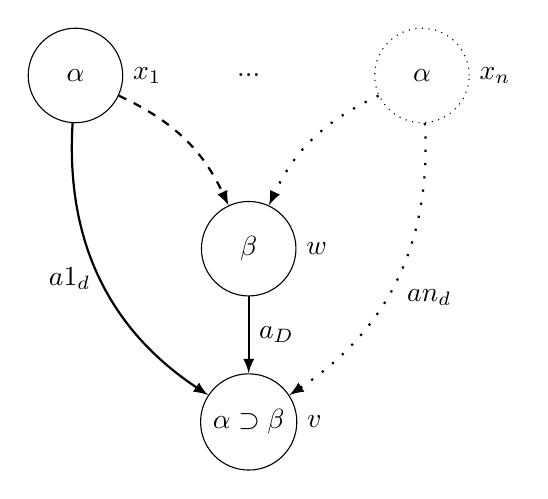
\begin{tikzpicture}[-triangle 60, node distance=2.2cm and 1cm, auto]
            % \tikzstyle{every state}=[circle,thick,minimum size=5mm, text=black,minimum width=1cm]
            \node[state, inner sep=1mm,minimum size=1.2cm, label=right:$x_1$] (A) {$\alpha$};
            \node[state, draw=none,fill=none] (D) [right of=A] {...};
            \node[state, inner sep=1mm,minimum size=1.2cm, dotted, label=right:$x_n$] (E) [right of=D] {$\alpha$};
            \node[state, inner sep=1mm,minimum size=1.2cm, label=right:$w$] (B) [below of=D] {$\beta$};
            \node[state, inner sep=1mm,minimum size=1.2cm, label=right:$v$] (C) [below of=B] {$\alpha \supset \beta$};
            
            \path[-latex]  (A) edge [bend right=30, thick, left]  node {{$a1_d$}} (C);
            \path[-latex]  (B) edge [thick] node {$a_D$} (C);
            \path[-latex]  (E) edge [bend left=30, loosely dotted, thick]  node {{$an_d$}} (C);
            \path[-latex]  (A) edge [bend left=20, dashed, thick] node {} (B);
            \path[-latex]  (E) edge [bend right=20, loosely dotted, thick] node {} (B);
        \end{tikzpicture}
    \end{center}
    
    o rótulo do vértice $w$ associado a $v$ por uma aresta de dedução ($a_D$) é idêntico ao consequente de $l(v)$; os rótulos dos vértices ($x_1, ..., x_n$) associados a $v$ por arestas de descarte ($a1_d, ..., an_d$) são idênticos ao antecedente de $l(v)$.
    
    \item Para todo vértice $v \in V$, se $ge(A_D, v) = 2$, então $l(v)$ é a conclusão de uma regra $\mysupset{-E}$, tal que
    
    \begin{center}
        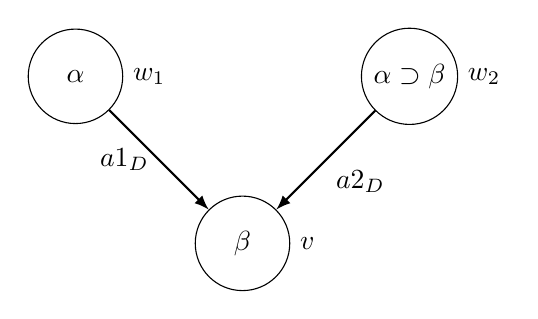
\begin{tikzpicture}[-triangle 60, node distance=3cm and 1cm, auto]
            % \tikzstyle{every state}=[circle,thick,minimum size=5mm, text=black,minimum width=1cm]
            \node[state, inner sep=1mm,minimum size=1.2cm, label=right:$v$] (A) {$\beta$};
            \node[state, inner sep=1mm,minimum size=1.2cm, label=right:$w_1$] (B) [above left of=A] {$\alpha$};
            \node[state, inner sep=1mm,minimum size=1.2cm, label=right:$w_2$] (C) [above right of=A] {$\alpha \supset \beta$};
            
            \path[-latex]  (B) edge [thick, left]  node {{$a1_D$}} (A);
            \path[-latex]  (C) edge [thick]  node {{$a2_D$}} (A);
        \end{tikzpicture}
    \end{center}
    
    sejam os vértices $w_1$ e $w_2$ associados a $v$, onde $|l(w_1)| < |l(w_2)|$, o rótulo de $w_1$ é idêntico ao antecedente de $l(w_2)$, o rótulo de $v$ é idêntico ao consequente de $l(w_2)$.
    
    \item Para todo vértice $v \in V$, se $ge(A_D, v) = 0$ e $gs(A_d, v) = 0$, então $l(v)$ é uma hipótese de $\Pi$.
\end{enumerate}
\end{definition}

Para exemplificar a representação de derivações por Grafos de Prova, a Figura \ref{fig:exe_gra_pro} mostra o grafo que representa a derivação de $$\vdash (A \supset (B \supset C)) \supset (B \supset (A \supset C))$$ As arestas com linhas tracejadas são arestas de descarte.

\begin{figure}[ht]
    \begin{center}
        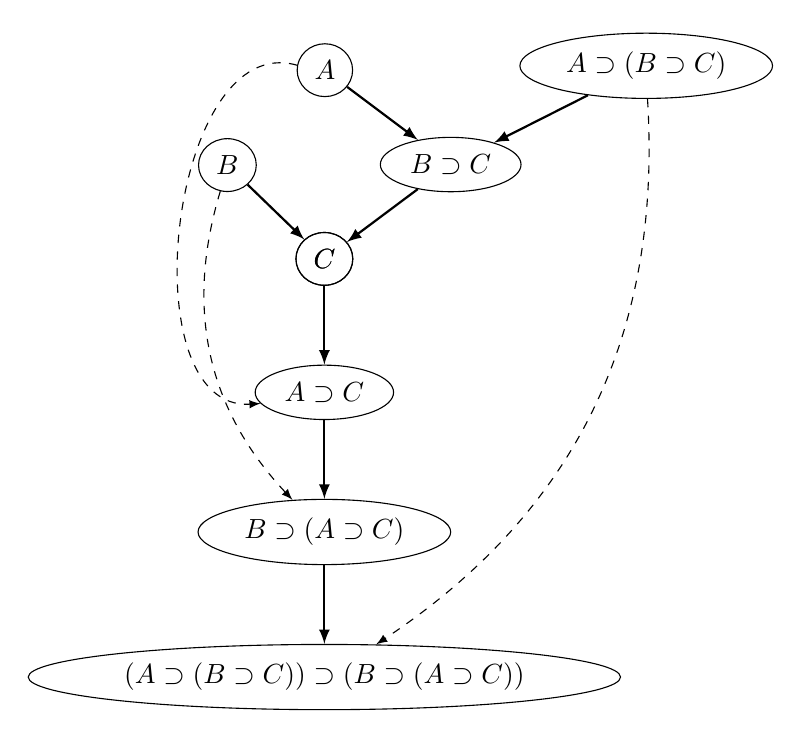
\begin{tikzpicture}[auto, elliptic state/.style={draw,ellipse}]
            % \tikzstyle{every state}=[circle,thick,minimum size=5mm, text=black,minimum width=1cm]
            \node[elliptic state] (ABCBAC) {$(A\supset(B\supset C)) \supset (B \supset (A\supset C))$};
            \node[elliptic state] (BAC) [above = 1cm of ABCBAC] {$B \supset (A\supset C)$};
            \node[elliptic state] (AC) [above = 1cm of BAC] {$A\supset C$};
            \node[elliptic state] (C) [above = 1cm of AC] {$C$};
            \node[elliptic state] (C) [above = 1cm of AC] {$C$};
            \node[elliptic state] (B) [above left = 1cm of C] {$B$};
            \node[elliptic state] (BC) [above right = 1cm of C] {$B\supset C$};
            \node[elliptic state] (ABC) [above right = 1cm of BC] {$A\supset(B\supset C)$};
            \node[elliptic state] (A) [above left = 1cm of BC] {$A$};
            
            % \node[state, inner sep=1mm,minimum size=1.2cm, label=right:$w_2$] (C) [above right of=A] {$\alpha \supset \beta$};
            
            \path[-latex]  (ABC) edge [thick] (BC);
            \path[-latex]  (A) edge [thick] (BC);
            \path[-latex]  (BC) edge [thick] (C);
            \path[-latex]  (B) edge [thick] (C);
            \path[-latex]  (C) edge [thick] (AC);
            \path[-latex]  (AC) edge [thick] (BAC);
            \path[-latex]  (BAC) edge [thick] (ABCBAC);
            
            \path[-latex]  (B) edge [dashed, bend right=30] (BAC);
            \path[-latex]  (A) edge [dashed, bend right=100] (AC);
            \path[-latex]  (ABC) edge [dashed, bend left=30] (ABCBAC);
        \end{tikzpicture}
    \end{center}
    \caption{Exemplo de grafo de derivação}
    \label{fig:exe_gra_pro}
\end{figure}

Seja uma derivação $\Pi$ de $\Gamma \vdash \alpha$, a conclusão $\alpha$ depende do conjunto de hipóteses $\Gamma$. Em um grafo de derivação que representa $\Pi$, o conjunto de hipóteses é composto pelos rótulos dos vértices que não possuem arestas de dedução incidentes e que não foram descartados por arestas de descarte. No entanto, as arestas de descarte ($A_d$) adicionam ciclos no grafo $\langle V, A_D \rangle$ (desconsiderando a direção das arestas). 

\begin{definition}
Seja uma derivação $\Pi$ de $\beta$ tendo o conjunto $\Gamma$ de hipóteses. Uma aplicação de $\mysupset{-I}$ é gulosa, se e somente se, produz $\alpha \supset \beta$ e descarta cada ocorrência não descartada de $\alpha$ em $\Pi$ na qual $\beta$ depende.
\end{definition}

\begin{lemma}
Seja uma derivação $\Pi$ de $\alpha$. A derivação $\Pi'$ resultante da transformação de todas as regras $\mysupset{-I}$ de $\Pi$ em gulosas ainda é uma derivação válida de $\alpha$ em M$\supset$ \cite{GorHaeHCNonPub}.
\end{lemma}

Com as regras $\mysupset{-I}$ gulosas, as informações de dependências podem ser diretamente determinadas nos vértices ($V$) ou nas arestas de dedução ($A_D$) e portanto, as arestas de descarte deixam de ser necessárias. As definições a seguir utilizam grafos de provas com todas as regras $\mysupset{-I}$ gulosas.

\vspace{3mm}

\begin{definition}
Seja $\Lambda$ um conjunto de fórmulas de tamanho $n$ e $\mathcal{O}(\Lambda)$ uma ordenação linear das fórmulas de $\Lambda$, $\mathcal{O}(\Lambda) = \{\beta_1, \beta_2, ..., \beta_n\}$. Uma cadeia de \textit{bits} em $\mathcal{O}(\Lambda)$ é uma sequência de \textit{bits} $\langle b_1, b_2, ..., b_n\rangle$, onde cada $b_i \in \{0, 1\}$ com $i$ variando de $1$ até $n$. Para todo conjunto de fórmulas $\Lambda$ de tamanho $n$, existe uma função bijetora $f$ entre o conjunto de todas as cadeias de bits de tamanho \textit{n} e o conjunto das partes de $\Lambda$, $f: B(\mathcal{O}(\Lambda)) \rightarrow \mathcal{P}(\Lambda)$, $f(\langle b_1, ..., b_n\rangle) = \{\beta_i | b_i = 1\}$.
\end{definition}

\begin{example}
Seja $\Lambda = \{A, B, C, (A \supset B)\}$ e uma ordenação linear  $\mathcal{O}(\Lambda) = [(A \supset B), A, C, B]$, onde $(A \supset B)$, $A$, $C$ e $B$ possuem os índices 1, 2, 3 e 4, respectivamente. Para cadeias de \textit{bits} de tamanho 4, a função $f$ da definição anterior possui o seguinte comportamento para as seguintes cadeias de \textit{bits}: $f(\langle 0, 1, 1, 0\rangle) = \{A, C\}$; $f(\langle 1, 0, 1, 0\rangle) = \{(A \supset B), C\}$.
\end{example}

Em uma derivação de $\Gamma \vdash \alpha$, sendo o conjunto $\Lambda = Sub
_{c}(\Gamma) \cup Sub_{f}(\alpha)$, $\mathcal{O}(\Lambda)$ pode ser utilizado para associar cada ocorrência de fórmula com suas respectivas dependências.

Na definição a seguir, considere $b_{\langle \beta \rangle}$ como a cadeia de \textit{bits} que contém apenas o \textit{bit} referente à fórmula $\beta$ igual a 1.

\vspace{3mm}

\begin{definition}{\textbf{Grafo de derivação decorado.}}
Sejam uma derivação $\Pi$ de $\Gamma \vdash \alpha$, um conjunto de fórmulas $\Lambda = Sub_{c}(\Gamma) \cup Sub_{f}(\alpha)$, um grafo de derivação de $\Pi$ $\langle V, A_D, A_d, r, c, l\rangle$ e uma ordenação linear $\mathcal{O}(\Lambda)$. $\langle V, A_D, r, c, l, d \rangle$ é um \textit{grafo de derivação decorado}, onde \textit{d} é uma função que associa cada aresta $(v1, v2) \in A_D$ a uma cadeia de bits que representa as dependências de $l(v1)$, $d: A_D \rightarrow B(\mathcal{O}(\Lambda))$, tal que:

\begin{enumerate}
    \item Para todo $v \in V$, se $v$ é uma hipótese e $l(v) = \alpha$, então $d(\langle v, v' \rangle) = b_{\langle \alpha \rangle}$ para algum $v' \in V$.
    
    \begin{center}
        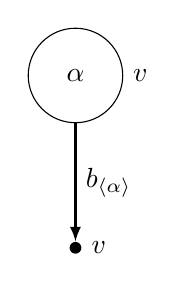
\begin{tikzpicture}[-triangle 60, node distance=3cm and 1cm, auto]
            \node[state, inner sep=1mm,minimum size=1.2cm, label=right:$v$] (A) {$\alpha$};
            \node[circle,fill,inner sep=1.5pt, label=right:$v$] (B) [below = 1.5cm of A] {};
            
            \path[-latex]  (A) edge [thick, right]  node {$b_{\langle \alpha \rangle}$} (B);
        \end{tikzpicture}
    \end{center}
    
    \item Para todo $v \in V$, se $v$ é a conclusão de uma regra $\mysupset{-E}$ e possui $w1, w2 \in V$ como premissas, onde $d(\langle w1, v \rangle) = \overrightarrow{b1}$ e $d(\langle w2, v \rangle) = \overrightarrow{b2}$, então $d(\langle v, v' \rangle) = \overrightarrow{b1} \oplus \overrightarrow{b2}$ para algum $v' \in V$.
    
    \begin{center}
        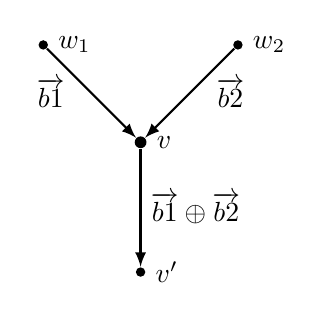
\begin{tikzpicture}[-triangle 60, node distance=3cm and 1cm, auto]
            % \tikzstyle{every state}=[circle,thick,minimum size=5mm, text=black,minimum width=1cm]
            \node[circle,fill,inner sep=1.5pt, label=right:$v$] (A) {};
            \node[circle,fill,inner sep=1.2pt, label=right:$w_1$] (B) [above left = 1.6cm of A] {};
            \node[circle,fill,inner sep=1.2pt, label=right:$w_2$] (C) [above right = 1.6cm of A] {};
            \node[circle,fill,inner sep=1.2pt, label=right:$v'$] (D) [below = 1.5cm of A] {};
            
            \path[-latex]  (B) edge [thick, left]  node[left=6pt] {$\overrightarrow{b1}$} (A);
            \path[-latex]  (C) edge [thick, right]  node[right=6pt] {$\overrightarrow{b2}$} (A);
            \path[-latex]  (A) edge [thick, right]  node {$\overrightarrow{b1} \oplus \overrightarrow{b2}$} (D);
        \end{tikzpicture}
    \end{center}
    
    \item Para todo $v \in V$, se $v$ é a conclusão de uma regra $\mysupset{-I}$, possui $l(v) =$ `$\alpha \supset \beta$' e $w \in V$ como premissa, onde $d(\langle w, v \rangle) = \overrightarrow{b1}$ e $l(w) = \alpha$, então $d(\langle v, v' \rangle) = \overrightarrow{b1} - b_{\langle \alpha \rangle}$ para algum $v' \in V$.
    
    \begin{center}
        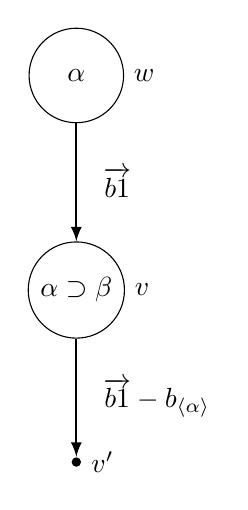
\begin{tikzpicture}[-triangle 60, node distance=3cm and 1cm, auto]
            % \tikzstyle{every state}=[circle,thick,minimum size=5mm, text=black,minimum width=1cm]
            \node[state, inner sep=1mm,minimum size=1.2cm, label=right:$v$] (A) {$\alpha \supset \beta$};
            \node[state, inner sep=1mm,minimum size=1.2cm, label=right:$w$] (B) [above = 1.5cm of A] {$\alpha$};
            \node[circle,fill,inner sep=1.2pt, label=right:$v'$] (C) [below = 1.5cm of A] {};
            
            \path[-latex]  (B) edge [thick, right]  node[right=6pt] {$\overrightarrow{b1}$} (A);
            \path[-latex]  (A) edge [thick, right]  node[right=6pt] {$\overrightarrow{b1} - b_{\langle \alpha \rangle}$} (C);
        \end{tikzpicture}
    \end{center}
\end{enumerate}

\end{definition}

A Figura \ref{fig:exe_gra_pro_dec} mostra um exemplo de grafo de derivação decorado obtido a partir do grafo de derivação da Figura \ref{fig:exe_gra_pro}. Considerando $$\alpha = (A\supset(B\supset C)) \supset (B \supset (A\supset C))$$ e ainda considerando $\Delta$ igual a $Sub_f(\alpha)$, onde $$Sub_f(\alpha)$$

\begin{figure}[ht]
    \begin{center}
        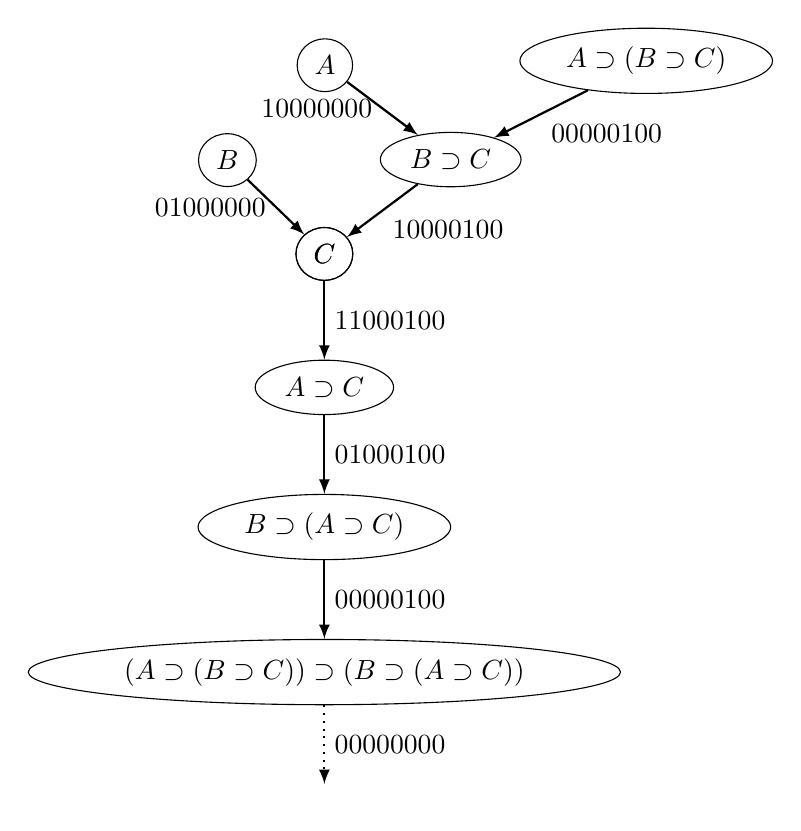
\begin{tikzpicture}[auto, elliptic state/.style={draw,ellipse}]
            % \tikzstyle{every state}=[circle,thick,minimum size=5mm, text=black,minimum width=1cm]
            \node[elliptic state] (ABCBAC) {$(A\supset(B\supset C)) \supset (B \supset (A\supset C))$};
            \node[elliptic state] (BAC) [above = 1cm of ABCBAC] {$B \supset (A\supset C)$};
            \node[elliptic state] (AC) [above = 1cm of BAC] {$A\supset C$};
            \node[elliptic state] (C) [above = 1cm of AC] {$C$};
            \node[elliptic state] (C) [above = 1cm of AC] {$C$};
            \node[elliptic state] (B) [above left = 1cm of C] {$B$};
            \node[elliptic state] (BC) [above right = 1cm of C] {$B\supset C$};
            \node[elliptic state] (ABC) [above right = 1cm of BC] {$A\supset(B\supset C)$};
            \node[elliptic state] (A) [above left = 1cm of BC] {$A$};
            \node[] (HN) [below = 1cm of ABCBAC] {};
            
            % \node[state, inner sep=1mm,minimum size=1.2cm, label=right:$w_2$] (C) [above right of=A] {$\alpha \supset \beta$};
            
            \path[-latex]  (ABC) edge [thick] node {00000100} (BC);
            \path[-latex]  (A) edge [thick, left] node {10000000} (BC);
            \path[-latex]  (BC) edge [thick] node {10000100} (C);
            \path[-latex]  (B) edge [thick, left] node {01000000} (C);
            \path[-latex]  (C) edge [thick] node {11000100} (AC);
            \path[-latex]  (AC) edge [thick] node {01000100} (BAC);
            \path[-latex]  (BAC) edge [thick] node {00000100} (ABCBAC);
            \path[-latex]  (ABCBAC) edge [thick, dotted] node {00000000} (HN);
        \end{tikzpicture}
    \end{center}
    \caption{Exemplo de grafo de derivação decorado}
    \label{fig:exe_gra_pro_dec}
\end{figure}

Um grafo de derivação decorado pode ser visto como uma árvore. A Compressão Horizontal ocorre em um grafo de derivação decorado fundindo os vértices que possuem rótulos idênticos e que estejam no mesmo nível da árvore. Durante a compressão, algumas informações adicionais são inseridas no grafo, essas informações são utilizadas para verificar se o grafo resultante da compressão corresponde a uma derivação válida. A seguir, definimos a estrutura do grafo de derivação utilizado pela Compressão Horizontal.

\vspace{3mm}

\begin{definition}{\textbf{Estrutura de grafo de derivação decorado (EGDD).}}
Seja $\Pi$ uma derivação de $\Gamma \vdash \alpha$, $\Delta = Sub_c(\Pi) \cup Sub_{f}(\alpha)$, um grafo de derivação decorado de $\Pi$ $\langle V, A_D, l, r, c, d \rangle$ e uma ordenação linear $\mathcal{O}(\Delta)$. $\langle V, A_D, A_A, r, l, g, d, p \rangle$ é uma EGDD, onde:

\begin{enumerate}
    \item $V$ é o conjunto não vazio de vértices.
    % \item $(A_{D}^{i})_{i \in \mathcal{O}(\Delta)}$ é o conjunto das famílias de arestas de dedução.
    \item $A_D$ é o conjunto das \textit{arestas de dedução}.
    \item $A_A \in V \times V$ é o conjunto das \textit{arestas de ancestralidade}.
    \item $l: V \rightarrow \Delta$ é a função que rotula os vértices com suas respectivas fórmulas em $\Pi$. 
    \item $r$ é a raiz de $\langle V, (A_{D}^{i})_{i \in \mathcal{O}(\Delta)} \rangle$, onde $l(r) = \alpha$.
    \item $g: A_D \rightarrow \{1, ...\; |\Delta|\}$ é a função de coloração das arestas de dedução. Cada elemento do conjunto $\{1, ...\; |\Delta|\}$ pode ser visto como uma cor para uma aresta de dedução.
    \item $d: \bigcup_{i \in \mathcal{O}(\Delta)} A_{D}^{i} \rightarrow  B(\mathcal{O}(\Delta))$ é a função que associa cada aresta de dedução $\langle v1, v2 \rangle$ à cadeia de bits que denota a dependência de $v1$. 
    \item $p: A_A \rightarrow \{1, ...\; |\Delta|\}^{\star}$, onde para cada aresta $\langle v1, v2 \rangle \in A_A$, $p(\langle v1, v2 \rangle)$ é uma cadeia de caracteres $\langle c_1, ..., c_n \rangle$, onde cada $c_i$, com $i = 1$ até $n$, é um índice da ordenação linear $\mathcal{O}(\Delta)$.
\end{enumerate}

\end{definition}

Antes de iniciar a compressão, a EGDD possui apenas arestas de dedução. Todas as arestas de dedução possuem cor 0 e todos os vértices possuem o grau de saída igual a 1, exceto a raiz, que possui grau de saída igual a 0.

\subsection{Algoritmo de compressão}

A Compressão Horizontal comprime a EGDD através da fusão de vértices rotulados com fórmulas idênticas que estejam no mesmo nível da árvore de derivação. Para cada fórmula em cada nível da árvore, uma estrutura de fila do tipo \textit{FIFO}\footnote{\textit{First In, First Out} - primeiro elemento inserido é o primeiro a ser removido.} contendo os vértices rotulados com a respectiva fórmula é criada. As fusões ocorrem com os vértices que estejam em uma fila com mais de um vértice. Em cada fila com mais de um elemento, os vértices são desenfileirados\footnote{Operação de remover um elemento da fila} e colapsados em pares. O colapso consiste na operação de remover dois vértices do grafo e adicionar um novo vértice, que é o resultante do colapso dos vértices removidos. O colapso sempre ocorre com pelo menos um vértice que ainda não foi colapsado. No caso de filas com mais de dois vértices, a partir do segundo, os colapsos ocorrem entre o vértice resultante do colapso anterior e um vértice retirado da fila. 

A Compressão Horizontal é executada pelo Algoritmo \ref{alg:comp_hor}. A função \textit{vérticesRótulosIdênticos} retorna uma lista de filas para cada fórmula presente em determinado nível da árvore de derivação. A função \textit{desenfileirar} executa a operação de remoção em uma fila.

\vspace{5mm}

\begin{algorithm}[H]
\label{alg:comp_hor}
\SetAlgoLined
\Entrada{EGDD}
\Saida{EGDD comprimida}
\Para{nível $=$ 1 até altura(G)}{
    vértices\_nível $\leftarrow$ \textit{vérticesRótulosIdênticos}(G, nível) \\
    \Para{vértices $\in$ vértices\_nível}{
        vértice\_1 $\leftarrow$ \textit{desenfileirar}(vértices) \\
        \Enqto{tamanho(vértices) $>$ 0}{
            vértice\_2 $\leftarrow$ \textit{desenfileirar}(vértices) \\
            vértice\_1 $\leftarrow$ \textit{colapsar}(vértice\_1, vértice\_2) \\
        }
    }
}
\caption{Compressão Horizontal}
\end{algorithm}

\vspace{5mm}

A função \textit{colapsar} recebe dois vértices, executa o colapso e retorna o vértice colapsado. Ao todo, a função possui 18 regras distintas para executar o colapso. A regra aplicada em cada colapso é determinada de acordo com as características dos vértices. A seguir, listamos e ilustramos as principais características dos vértices consideradas no momento do colapso:

\begin{itemize}
    \item \textbf{Arestas de ancestralidade} \\
    Ao colapsar dois vértices, as premissas de ambos os vértices passam a apontar para o vértice colapsado. As arestas de ancestralidade servem para identificar as premissas após o colapso, que são adicionadas somente se o vértice possui premissa(s) antes do colapso.
    
    \begin{center}
        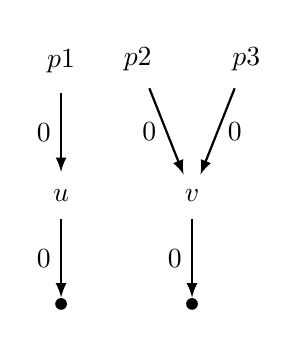
\begin{tikzpicture}[state/.style={circle}]
            % \tikzstyle{every state}=[circle,thick,minimum size=5mm, text=black,minimum width=1cm]
            \node[circle,fill,inner sep=1.5pt] (su) {};
            \node[state] (u) [above = 1cm of su] {$u$};
            \node[state] (p1) [above = 1cm of u] {$p1$};
            
            \node[circle,fill,inner sep=1.5pt] (sv) [right = 1.5cm of su] {};
            \node[state] (v) [above = 1cm of sv] {$v$};
            \node[state] (p2) [above left = 1.25cm and 0.2cm of v] {$p2$};
            \node[state] (p3) [above right = 1.25cm and 0.2cm of v] {$p3$};
            
            \path[-latex]  (p1) edge [thick, left] node {0} (u);
            \path[-latex]  (u) edge [thick, left] node {0} (su);
            \path[-latex]  (p2) edge [thick, left] node {0} (v);
            \path[-latex]  (p3) edge [thick, right] node {0} (v);
            \path[-latex]  (v) edge [thick, left] node {0} (sv);
        \end{tikzpicture}
        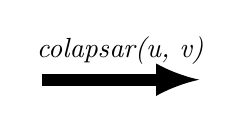
\begin{tikzpicture}
            \draw[-latex, thick, line width=1.5mm, above] (0,.5) -- node {\textit{colapsar(u, v)}} (2,.5);
        \end{tikzpicture}
        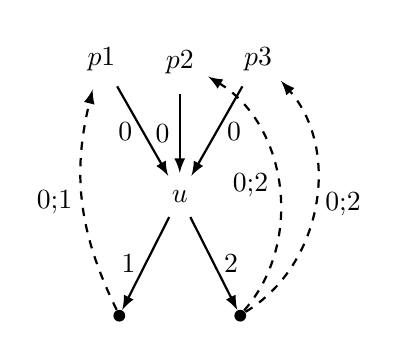
\begin{tikzpicture}[state/.style={circle}]
            % \tikzstyle{every state}=[circle,thick,minimum size=5mm, text=black,minimum width=1cm]
            \node[state] (u) {$u$};
            \node[circle,fill,inner sep=1.5pt] (su) [below left = 1.25cm and 0.5cm of u] {};
            \node[circle,fill,inner sep=1.5pt] (sv) [below right = 1.25cm and 0.5cm of u] {};
            \node[state] (p1) [above left = 1.25cm and 0.5cm of u] {$p1$};
            \node[state] (p2) [above = 1cm of u] {$p2$};
            \node[state] (p3) [above right = 1.25cm and 0.5cm of u] {$p3$};
            
            \path[-latex]  (p1) edge [thick, left] node {0} (u);
            \path[-latex]  (u) edge [thick, left] node {1} (su);
            \path[-latex]  (p2) edge [thick, left] node {0} (u);
            \path[-latex]  (p3) edge [thick, right] node {0} (u);
            \path[-latex]  (u) edge [thick, right] node {2} (sv);
            \path[-latex]  (su) edge [thick, left, dashed, bend left=20] node {0;1} (p1);
            \path[-latex]  (sv) edge [thick, left, dashed, bend right=50] node {0;2} (p2);
            \path[-latex]  (sv) edge [thick, right, dashed, bend right=50] node {0;2} (p3);
        \end{tikzpicture}
    \end{center}
    
    \begin{center}
        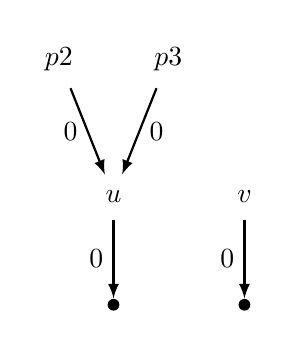
\begin{tikzpicture}[state/.style={circle}]
            % \tikzstyle{every state}=[circle,thick,minimum size=5mm, text=black,minimum width=1cm]
            \node[circle,fill,inner sep=1.5pt] (su) {};
            \node[state] (u) [above = 1cm of su] {$u$};
            \node[state] (p1) [above left = 1.25cm and 0.2cm of u] {$p2$};
            \node[state] (p2) [above right = 1.25cm and 0.2cm of u] {$p3$};
            
            \node[circle,fill,inner sep=1.5pt] (sv) [right = 1.5cm of su] {};
            \node[state] (v) [above = 1cm of sv] {$v$};
            
            \path[-latex]  (p1) edge [thick, left] node {0} (u);
            \path[-latex]  (u) edge [thick, left] node {0} (su);
            \path[-latex]  (p2) edge [thick, right] node {0} (u);
            \path[-latex]  (v) edge [thick, left] node {0} (sv);
        \end{tikzpicture}
        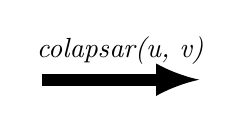
\begin{tikzpicture}
            \draw[-latex, thick, line width=1.5mm, above] (0,.5) -- node {\textit{colapsar(u, v)}} (2,.5);
        \end{tikzpicture}
        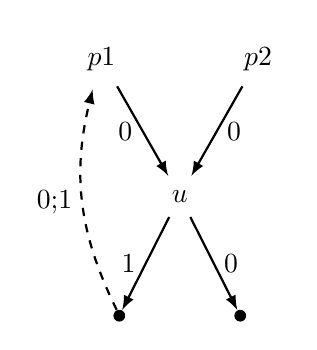
\begin{tikzpicture}[state/.style={circle}]
            % \tikzstyle{every state}=[circle,thick,minimum size=5mm, text=black,minimum width=1cm]
            \node[state] (u) {$u$};
            \node[circle, fill, inner sep=1.5pt] (su) [below left = 1.25cm and 0.5cm of u] {};
            \node[circle, fill, inner sep=1.5pt] (sv) [below right = 1.25cm and 0.5cm of u] {};
            \node[state] (p1) [above left = 1.25cm and 0.5cm of u] {$p1$};
            \node[state] (p2) [above right = 1.25cm and 0.5cm of u] {$p2$};
            
            \path[-latex]  (p1) edge [thick, left] node {0} (u);
            \path[-latex]  (u) edge [thick, left] node {1} (su);
            \path[-latex]  (p2) edge [thick, right] node {0} (u);
            \path[-latex]  (u) edge [thick, right] node {0} (sv);
            \path[-latex]  (su) edge [thick, left, dashed, bend left=20] node {0;1} (p1);
        \end{tikzpicture}
    \end{center}
    
    Cada aresta de ancestralidade possui como rótulo a informação necessária para refazer o caminho entre o destino e a origem através das arestas de dedução, esse caminho é identificado através das cores das arestas de dedução. Se o vértice possui premissas antes do colapso, é necessário atribuir uma cor para sua respectiva aresta dedutiva de saída após o colapso. Todas as arestas de dedução que saem de um determinado vértice possuem cores distintas, exceto para a cor 0.
    
    \item \textbf{Arestas de ancestralidade incidentes} \\
    Caso algum dos vértices a serem colapsados possua uma aresta de ancestralidade incidente, é necessário atualizar o destino e consequentemente o rótulo da aresta. Se o vértice possuir premissas, a aresta de ancestralidade é redirecionada para as premissas, caso contrário, a aresta é redirecionada para o vértice imediatamente inferior.
    
    \begin{center}
        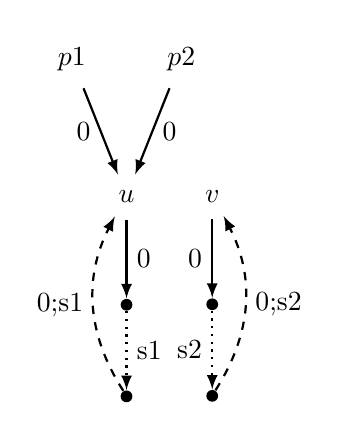
\begin{tikzpicture}[state/.style={circle}]
            % \tikzstyle{every state}=[circle,thick,minimum size=5mm, text=black,minimum width=1cm]
            \node[state] (u) {$u$};
            \node[state] (v) [right = 0.5cm of u] {$v$};
            
            \node[state] (p1) [above left = 1.25cm and 0.2cm of u] {$p1$};
            \node[state] (p2) [above right = 1.25cm and 0.2cm of u] {$p2$};
            \node[circle,fill,inner sep=1.5pt] (su) [below = 1cm of u] {};
            \node[circle,fill,inner sep=1.5pt] (ssu) [below = 1cm of su] {};
            
            \node[circle,fill,inner sep=1.5pt] (sv) [below = 1cm of v] {};
            \node[circle,fill,inner sep=1.5pt] (ssv) [below = 1cm of sv] {};
            
            \path[-latex]  (p1) edge [thick, left] node {0} (u);
            \path[-latex]  (p2) edge [thick, right] node {0} (u);
            \path[-latex]  (u) edge [thick, right] node {0} (su);
            \path[-latex]  (su) edge [thick, dotted, right] node {s1} (ssu);
            \path[-latex]  (ssu) edge [thick, dashed, left, bend left = 30] node {0;s1} (u);
            
            \path[-latex]  (v) edge [thick, left] node {0} (sv);
            \path[-latex]  (sv) edge [thick, dotted, left] node {s2} (ssv);
            \path[-latex]  (ssv) edge [thick, dashed, right, bend right = 30] node {0;s2} (v);
        \end{tikzpicture}
        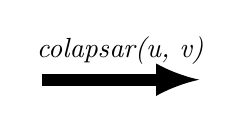
\begin{tikzpicture}
            \draw[-latex, thick, line width=1.5mm, above] (0,.5) -- node {\textit{colapsar(u, v)}} (2,.5);
        \end{tikzpicture}
        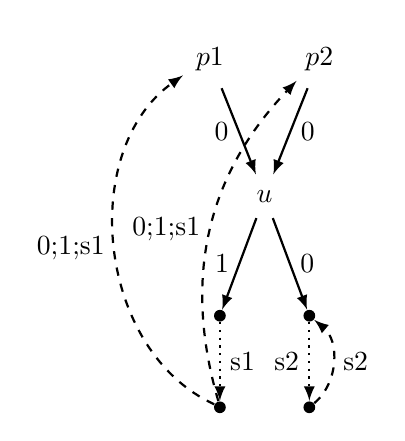
\begin{tikzpicture}[state/.style={circle}]
            % \tikzstyle{every state}=[circle,thick,minimum size=5mm, text=black,minimum width=1cm]
            \node[state] (u) {$u$};
            
            \node[state] (p1) [above left = 1.25cm and 0.2cm of u] {$p1$};
            \node[state] (p2) [above right = 1.25cm and 0.2cm of u] {$p2$};
            \node[circle,fill,inner sep=1.5pt] (su) [below left = 1.25cm and 0.3cm of u] {};
            \node[circle,fill,inner sep=1.5pt] (ssu) [below = 1cm of su] {};
            
            \node[circle,fill,inner sep=1.5pt] (sv) [below right = 1.25cm and 0.3cm of u] {};
            \node[circle,fill,inner sep=1.5pt] (ssv) [below = 1cm of sv] {};
            
            \path[-latex]  (p1) edge [thick, left] node {0} (u);
            \path[-latex]  (p2) edge [thick, right] node {0} (u);
            \path[-latex]  (u) edge [thick, left] node {1} (su);
            \path[-latex]  (su) edge [thick, dotted, right] node {s1} (ssu);
            \path[-latex]  (ssu) edge [thick, dashed, left, bend left = 60] node {0;1;s1} (p1);
            \path[-latex]  (ssu) edge [thick, dashed, left, bend left = 30] node {0;1;s1} (p2);
            
            \path[-latex]  (u) edge [thick, right] node {0} (sv);
            \path[-latex]  (sv) edge [thick, dotted, left] node {s2} (ssv);
            \path[-latex]  (ssv) edge [thick, dashed, right, bend right = 50] node {s2} (sv);
        \end{tikzpicture}
    \end{center}
    
    \item \textbf{Colapso de arestas} \\
    Nem sempre os destinos das arestas de dedução que saem dos vértices a serem colapsados possuem destinos diferentes. Caso os destinos já tenham sido colapsados no nível inferior, além de colapsar os vértices, é necessário colapsar as arestas.
    
    \begin{center}
        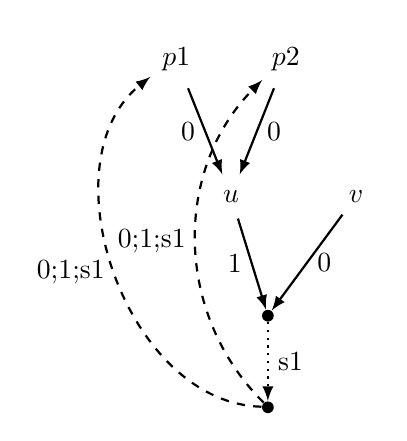
\begin{tikzpicture}[state/.style={circle}]
            % \tikzstyle{every state}=[circle,thick,minimum size=5mm, text=black,minimum width=1cm]
            \node[state] (u) {$u$};
            \node[state] (v) [right = 1cm of u] {$v$};
            
            \node[state] (p1) [above left = 1.25cm and 0.2cm of u] {$p1$};
            \node[state] (p2) [above right = 1.25cm and 0.2cm of u] {$p2$};
            \node[circle,fill,inner sep=1.5pt] (s) [below right = 1.25cm and 0.2cm of u] {};
            \node[circle,fill,inner sep=1.5pt] (ssu) [below = 1cm of s] {};
            
            \path[-latex]  (p1) edge [thick, left] node {0} (u);
            \path[-latex]  (p2) edge [thick, right] node {0} (u);
            \path[-latex]  (u) edge [thick, left] node {1} (s);
            \path[-latex]  (s) edge [thick, dotted, right] node {s1} (ssu);
            \path[-latex]  (ssu) edge [thick, dashed, left, bend left = 70] node {0;1;s1} (p1);
            \path[-latex]  (ssu) edge [thick, dashed, left, bend left = 45] node {0;1;s1} (p2);
            
            \path[-latex]  (v) edge [thick, right] node {0} (s);
        \end{tikzpicture}
        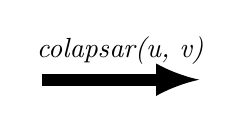
\begin{tikzpicture}
            \draw[-latex, thick, line width=1.5mm, above] (0,.5) -- node {\textit{colapsar(u, v)}} (2,.5);
        \end{tikzpicture}
        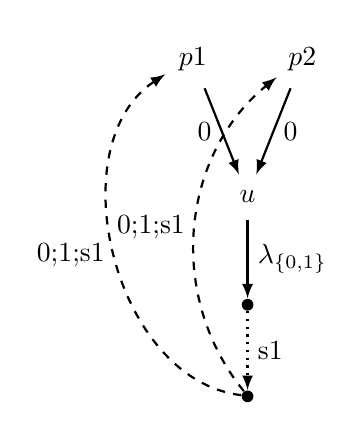
\begin{tikzpicture}[state/.style={circle}]
            % \tikzstyle{every state}=[circle,thick,minimum size=5mm, text=black,minimum width=1cm]
            \node[state] (u) {$u$};
            
            \node[state] (p1) [above left = 1.25cm and 0.2cm of u] {$p1$};
            \node[state] (p2) [above right = 1.25cm and 0.2cm of u] {$p2$};
            \node[circle,fill,inner sep=1.5pt] (s) [below = 1cm of u] {};
            \node[circle,fill,inner sep=1.5pt] (ssu) [below = 1cm of s] {};
            
            \path[-latex]  (p1) edge [thick, left] node {0} (u);
            \path[-latex]  (p2) edge [thick, right] node {0} (u);
            \path[-latex]  (u) edge [thick, right] node {$\lambda_{\{0,1\}}$} (s);
            \path[-latex]  (s) edge [thick, dotted, right] node {s1} (ssu);
            \path[-latex]  (ssu) edge [thick, dashed, left, bend left = 70] node {0;1;s1} (p1);
            \path[-latex]  (ssu) edge [thick, dashed, left, bend left = 45] node {0;1;s1} (p2);
        \end{tikzpicture}
    \end{center}
    
    $\lambda$ é a cor especial utilizada para indicar que a aresta foi colapsada. As arestas colapsadas ainda mantêm a informação das cores originais das arestas.
    
\end{itemize}

% \section{Dedução Natural Contextual}

% Proposta por Paleo em \cite{NDcPaleo}, a Dedução Natural Contextual (DNc) é um cálculo de dedução natural para M$\supset$ que utiliza \textit{deep inference}, o que permite aplicar as regras de dedução diretamente nas subfórmulas. Para alguns teoremas, a DNc é capaz de gerar provas quadraticamente menores que a dedução natural usual. Levando em consideração o isomorfismo de Curry-Howard entre a dedução natural da lógica intuicionista e o $\lambda$-$calculus$ simplesmente tipado, NDc é definido através do $\lambda_{c}$-$calculus$, uma extensão do $\lambda$-$calculus$ simplesmente tipado.

% Proposto por Alonzo Church em 1940, o $\lambda$-$calculus$ é um sistema formal voltado para a representação de funções computáveis.

% \begin{definition}{\textbf{$\lambda$-termos.}}
% Seja um conjunto infinito de variáveis $\{x, y, ...\}$, o conjunto de $\lambda$-termos é definido como segue:

% \begin{enumerate}
%     \item Toda variável é um $\lambda$-termo.
%     \item Se $x$ é uma variável e A é um $\lambda$-termo, $\lambda{x}.A$ é um $\lambda$-termo.
%     \item Se A e B são $\lambda$-termos, $(A B)$ é um $\lambda$-termo.
% \end{enumerate}
% \end{definition}

% Em sua versão tipada, cada termo do $\lambda$-$calculus$ possui um tipo associado. Seja o conjunto de variáveis de tipos $\{\alpha, \beta, ...\}$, as \textit{declarações de tipos} $$t:\alpha$$ $$t^{\alpha}$$ declaram que o termo $t$ possui o tipo $\alpha$, e $$t: \alpha \rightarrow \beta$$ declara que $t$ é uma função que transforma um argumento do tipo $\alpha$ em um argumento do tipo $\beta$. Os tipos de cada termo são definidos através das \textit{regras de tipagem} utilizando as \textit{relações de tipagem}. A relação de tipagem $$\Gamma \vdash t: \alpha$$ informa que no contexto de tipagem $\Gamma$ o termo $t$ possui tipo $\alpha$, o contexto de tipagem $\Gamma$ é um conjunto de declarações de tipos. Seja $\mathcal{I}$ um isomorfismo entre o $\lambda$-$calculus$ simplesmente tipado e a dedução natural de M$\supset$, onde um $\lambda$-termo com tipo $\alpha$ corresponde a prova do teorema $\alpha$ em M$\supset$, as regras de inferência da dedução natural de M$\supset$ correspondem as regras de tipagem do $\lambda$-$calculus$ simplesmente tipado (Figura \ref{fig:tip_lambda}).

% \begin{figure}[ht]
%     \begin{center}
%         \begin{minipage}[t][25mm][t]{130mm}
%             \begin{prooftree}
%                 \AxiomC{}
%                 \UnaryInfC{$\Gamma, a: \alpha \vdash a: \alpha$}
%             \end{prooftree}
%         \end{minipage}
%         \begin{minipage}[t][25mm][t]{65mm}
%             \begin{prooftree}
%                 \AxiomC{$\Gamma, a: \alpha \vdash b: \beta$}
%                 \RightLabel{$\mysupset{-I}$}
%                 \UnaryInfC{$\Gamma \vdash \lambda{a^{\alpha}}.b: \alpha \rightarrow \beta$}
%             \end{prooftree}
%         \end{minipage}
%         \hfill
%         \begin{minipage}[t][25mm][t]{65mm}
%             \begin{prooftree}
%                 \AxiomC{$\Gamma \vdash f: \alpha \rightarrow \beta$}
%                 \AxiomC{$\Gamma \vdash a: \alpha$}
%                 \RightLabel{$\mysupset{-E}$}
%                 \BinaryInfC{$\Gamma \vdash (f a): \beta$}
%             \end{prooftree}
%         \end{minipage}
%     \caption{Regras de tipagem (inferência) do $\lambda$-$calculus$ simplesmente tipado (da dedução natural para M$\supset$)}
%     \label{fig:tip_lambda}
%     \end{center}
% \end{figure}

% A DNc aplica as regras de inferência diretamente nas subfórmulas. Seja $\alpha$ uma fórmula, $\mathcal{C}_{\pi}[\alpha]$ representa a subfórmula de $\alpha$ na posição $\pi$, $\mathcal{C}_{\pi}[\_]$ é o contexto de $\alpha$. Seja uma representação em árvore binária da fórmula $\alpha$, onde cada implicação é uma ramificação, a posição $\pi$ é representada por uma cadeia de \textit{bits} que representa o caminho da raiz de $\mathcal{C}_{\pi}[\alpha]$ até $\alpha$. As regras de inferência da DNc são mostradas na Figura \ref{fig:tip_DNc}.

% \begin{figure}[ht]
%     \begin{center}
%         \begin{minipage}[t][25mm][t]{130mm}
%             \begin{prooftree}
%                 \AxiomC{}
%                 \UnaryInfC{$\Gamma, a: \alpha \vdash a: \alpha$}
%             \end{prooftree}
%         \end{minipage}
%         \begin{minipage}[t][25mm][t]{130mm}
%             \begin{prooftree}
%                 \AxiomC{$\Gamma, a: \alpha \vdash b: \mathcal{C_{\pi}}[\beta$]}
%                 \RightLabel{$\mysupset{-I}$}
%                 \UnaryInfC{$\Gamma \vdash \lambda{a^{\alpha}}.b: \mathcal{C_{\pi}}[\alpha \rightarrow \beta]$}
%             \end{prooftree}
%         \end{minipage}
%         \hfill
%         \begin{minipage}[t][25mm][t]{130mm}
%             \begin{prooftree}
%                 \AxiomC{$\Gamma \vdash f: \mathcal{C}_{\pi1}^1[\alpha \rightarrow \beta]$}
%                 \AxiomC{$\Gamma \vdash a: \mathcal{C}_{\pi2}^2[\alpha]$}
%                 \RightLabel{$\mysupset{-E^\rightharpoonup}$}
%                 \BinaryInfC{$\Gamma \vdash (f$ $a)_{(\pi1;\pi2)}^{\rightharpoonup}: \mathcal{C}_{\pi1}^1[\mathcal{C}_{\pi2}^2[\beta]]$}
%             \end{prooftree}
%         \end{minipage}
%         \begin{minipage}[t][25mm][t]{130mm}
%             \begin{prooftree}
%                 \AxiomC{$\Gamma \vdash f: \mathcal{C}_{\pi1}^1[\alpha \rightarrow \beta]$}
%                 \AxiomC{$\Gamma \vdash a: \mathcal{C}_{\pi2}^2[\alpha]$}
%                 \RightLabel{$\mysupset{-E^\leftharpoonup}$}
%                 \BinaryInfC{$\Gamma \vdash (f$ $a)_{(\pi1;\pi2)}^{\leftharpoonup}: \mathcal{C}_{\pi2}^2[\mathcal{C}_{\pi1}^1[\beta]]$}
%             \end{prooftree}
%         \end{minipage}
%     \caption{Regras de tipagem (inferência) do $\lambda_{c}$-$calculus$ (da DNc)}
%     \label{fig:tip_DNc}
%     \end{center}
% \end{figure}

% Existem duas regras de eliminação da implicação, uma para cada possibilidade de combinação dos contextos. Essa peculiaridade pode tornar a implementação de provadores de teoremas para NDc mais complexas e, consequentemente, mais lentas.

% A completude e a corretude são mostradas através de traduções em ambos os sentidos de provas de teoremas em dedução natural usal e NDc, os detalhes dessas traduções não fazem parte do escopo deste trabalho.

% \section{Compressão de Dados}

\section{Codificação de Huffman}

Proposta em 1952 por David Huffman \cite{huffman1952}, a \textit{Codificação de Huffman} é uma técnica de compressão de dados sem perdas, que permite recuperar o dado original a partir do dado comprimido, baseada na substituição de símbolos do dado por códigos. O objetivo é minimizar a quantidade de espaço necessário para representar o dado atribuindo códigos menores para os símbolos mais frequentes e códigos maiores para os menos frequentes. Para otimizar o uso do espaço, normalmente, utiliza-se uma codificação binária para comprimir os dados, no entanto, a codificação de Huffman é extensível para codificações n-árias. 

\theoremstyle{definition}
\begin{definition}{\textbf{Codificação binária.}}
Seja uma mensagem \textit{m} com um alfabeto $\Sigma$, uma \textit{codificação binária} é uma função $F$ que mapeia cada símbolo de $\Sigma$ em uma cadeia de bits, $F: \Sigma \rightarrow \{0, 1\}^*$, tal que:

\begin{enumerate}
    \item Para todo símbolo $a \in \Sigma$, $F(a) \neq \epsilon$, $F(a)$ não é vazia.
    \item Para todos símbolos $a, b \in \Sigma$, $F(a) \neq F(b)$.
    \item Para todos símbolos $a, b \in \Sigma$, $F(a)$ não é prefixo de $F(b)$.
\end{enumerate}
\end{definition}

A condição (3) permite que, dada uma mensagem $m = \langle a_1, ..., a_n \rangle$ e uma codificação binária $F$, a mensagem codificada $m_c = \langle F(a_1), ..., F(a_n) \rangle$ seja decodificada sem informações adicionais. Por exemplo, seja uma mensagem $babcb$ e uma codificação binária, $F(a) = 111$, $F(b) = 010$ e $F(c) = 000$. Uma mensagem codificada $010111010000010$ possui apenas uma segmentação possível baseada na codificação binária do alfabeto, $010|111|010|000|010$, que corresponde exatamente a mensagem original $babcb$.

A construção da codificação binária utilizada por Huffman é baseada na probabilidade de ocorrência dos símbolos do alfabeto na mensagem a ser codificada, utilizando tabelas auxiliares para atribuir códigos a cada símbolo do alfabeto. Seja $(s, p)$, um símbolo e sua respectiva probabilidade de ocorrência, a construção das tabelas auxiliares segue os seguintes passos:

\begin{enumerate}
    \item Inicialmente, uma tabela com todos os símbolos e suas respectivas probabilidades é criada, as entradas são ordenadas em ordem decrescente das probabilidades.
    \item Seleciona as entradas com as menores probabilidades, $(s_1, p_1)$ e $(s_2, p_2)$, cria uma entrada auxiliar $((s_1, s_2), p_1+p_2)$ e adiciona em uma nova tabela com as entradas de todos os símbolos, exceto $s_1$ e $s_2$.
    \item Repete o passo 2 até que a tabela criada tenha apenas uma entrada.
\end{enumerate}

A Figura \ref{fig:exe_tab_aux} mostra um exemplo de criação das tabelas auxiliares do alfabeto $\Sigma = \{a, r, j, l, m, p\}$, onde as probabilidades de $a, r, j, l, m$ e $p$ são, respectivamente, 0.35, 0.20, 0.15, 0.13, 0.12 e 0.05. Para facilitar a visualização, as entradas auxiliares estão destacadas em negrito.

\begin{figure}[ht]
    \begin{center}
        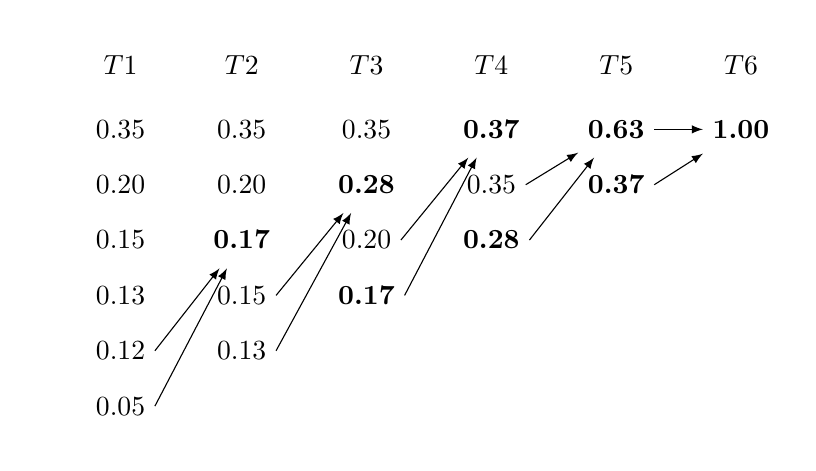
\begin{tikzpicture}
        [every node/.style={minimum height=2em}]
        \matrix [matrix of math nodes](Mat)
        {
        |[minimum width=1.8em]|& T1 &|[minimum width=1.8em]| & T2 &|[minimum width=1.8em]|& T3 &|[minimum width=1.8em]|& T4 &|[minimum width=1.8em]|& T5 &|[minimum width=1.8em]|& T6\\
        & 0.35 && 0.35           && 0.35          && \textbf{0.37} && \textbf{0.63} && \textbf{1.00}\\
        & 0.20 && 0.20           && \textbf{0.28} && 0.35          && \textbf{0.37} &&     \\
        & 0.15 && \textbf{0.17}  && 0.20          && \textbf{0.28} &&               &&     \\
        & 0.13 && 0.15           && \textbf{0.17} &&               &&               &&     \\
        & 0.12 && 0.13           &&               &&               &&               &&     \\
        & 0.05 && &              &&               &&               &&               &&     \\
        };
        
        \draw[-latex] (Mat-7-2.east) -- (Mat-4-4);
        \draw[-latex] (Mat-6-2.east) -- (Mat-4-4);
        \draw[-latex] (Mat-5-4.east) -- (Mat-3-6);
        \draw[-latex] (Mat-6-4.east) -- (Mat-3-6);
        \draw[-latex] (Mat-4-6.east) -- (Mat-2-8);
        \draw[-latex] (Mat-5-6.east) -- (Mat-2-8);
        \draw[-latex] (Mat-3-8.east) -- (Mat-2-10);
        \draw[-latex] (Mat-4-8.east) -- (Mat-2-10);
        \draw[-latex] (Mat-2-10.east) -- (Mat-2-12);
        \draw[-latex] (Mat-3-10.east) -- (Mat-2-12);
        \end{tikzpicture}
        \caption{Exemplo de tabelas auxiliares da codificação de Huffman}
        \label{fig:exe_tab_aux}
    \end{center}
\end{figure}

A partir das tabelas auxiliares é possível construir uma árvore binária para a obtenção do código de cada símbolo, tal construção ocorre percorrendo as tabelas na direção inversa da criação, onde a raiz da árvore é a entrada auxiliar com probabilidade igual a 1.0 da última tabela e as folhas são as entradas originais (tabela T1) das probabilidades dos símbolos do alfabeto. Para cada fusão de entradas realizada pelo passo 2 é criada uma ramificação na árvore, onde a entrada com a menor probabilidade é atribuída ao filho direito e a entrada com maior probabilidade é atribuída ao filho esquerdo. Cada arco da árvore é rotulado com 1 ou 0, os arcos dos filhos esquerdos e direitos são rotulados, respectivamente, com 0 e 1. A Figura \ref{fig:exe_arv_bin} mostra a árvore criada a partir das tabelas da Figura \ref{fig:exe_tab_aux}.

\begin{figure}[!ht]
    \begin{center}
        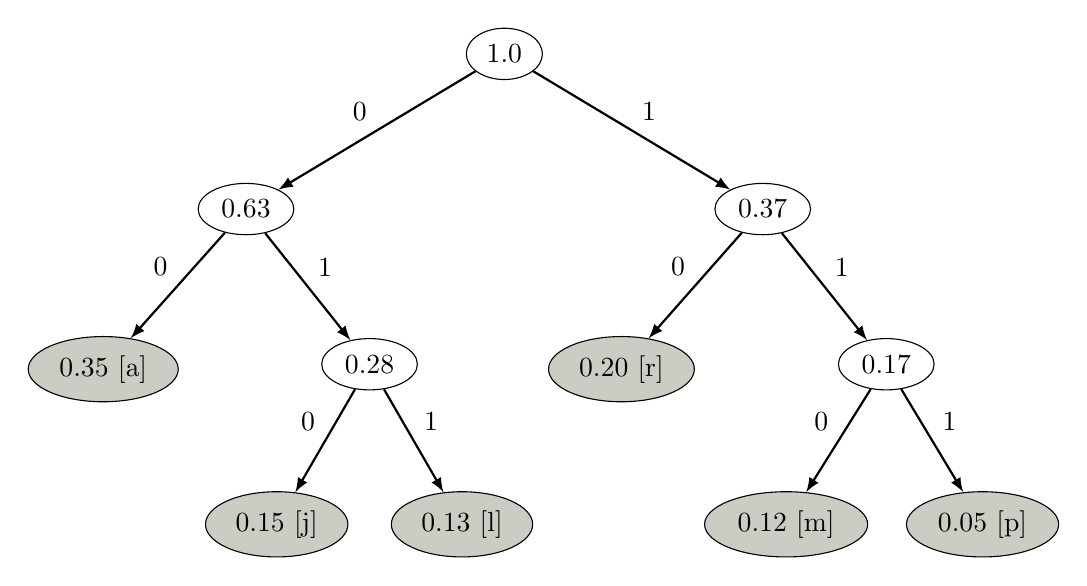
\begin{tikzpicture}[auto, elliptic state/.style={draw,ellipse}]
            % \tikzstyle{every state}=[circle,thick,minimum size=5mm, text=black,minimum width=1cm]
            \node[elliptic state] (root) {1.0};
            \node[elliptic state] [below left = 1.5cm and 2.5cm of root] (l) {0.63};
            \node[elliptic state, fill = backcolour2] (ll) [below left = 1.5cm and 0.7cm of l] {0.35 [a]};
            \node[elliptic state] (lr) [below right = 1.5cm and 0.7cm of l] {0.28};
            \node[elliptic state, fill = backcolour2] (lrl) [below left = 1.5cm and 0.1cm of lr] {0.15 [j]};
            \node[elliptic state, fill = backcolour2] (lrr) [below right = 1.5cm and 0.1cm of lr] {0.13 [l]};
            \node[elliptic state] (r) [below right = 1.5cm and 2.5cm of root] {0.37};
            \node[elliptic state, fill = backcolour2] (rl) [below left = 1.5cm and 0.7cm of r] {0.20 [r]};
            \node[elliptic state] (rr) [below right = 1.5cm and 0.7cm of r] {0.17};
            \node[elliptic state, fill = backcolour2] (rrl) [below left = 1.5cm and 0.1cm of rr] {0.12 [m]};
            \node[elliptic state, fill = backcolour2] (rrr) [below right = 1.5cm and 0.1cm of rr] {0.05 [p]};
            
            % \node[state, inner sep=1mm,minimum size=1.2cm, label=right:$w_2$] (C) [above right of=A] {$\alpha \supset \beta$};
            
            \path[-latex]  (root) edge [thick, above left] node {0} (l);
            \path[-latex]  (root) edge [thick] node {1} (r);
            \path[-latex]  (l) edge [thick] node {1} (lr);
            \path[-latex]  (l) edge [thick, above left] node {0} (ll);
            \path[-latex]  (lr) edge [thick, above left] node {0} (lrl);
            \path[-latex]  (lr) edge [thick] node {1} (lrr);
            \path[-latex]  (r) edge [thick] node {1} (rr);
            \path[-latex]  (r) edge [thick, above left] node {0} (rl);
            \path[-latex]  (rr) edge [thick, above left] node {0} (rrl);
            \path[-latex]  (rr) edge [thick] node {1} (rrr);
        \end{tikzpicture}
        \caption{Exemplo de árvore binária criada a partir das tabelas auxiliares da codificação de Huffman}
        \label{fig:exe_arv_bin}
    \end{center}
\end{figure}

Os códigos de cada símbolo são obtidos percorrendo os caminhos da raiz até cada folha e armazenando os rótulos dos arcos percorridos. A Tabela \ref{tab:cod_huf} mostra os códigos obtidos da árvore da Figura \ref{fig:exe_arv_bin}. Os símbolos com as maiores probabilidades, 'a' e 'r', ficaram com os menores códigos, respectivamente, 00 e 10. 

\begin{table} [!ht]
    \caption{Exemplos de códigos obtidos a partir da árvore binária da codificação de Huffman.}\label{tab:cod_huf}
    ~\\[-2mm]
    \begin{tabularx}{\textwidth}{@{\extracolsep{0pt}}C @{\extracolsep{0pt}}C C C}

        \textbf{Símbolo}
        & \textbf{Probabilidade}
        & \textbf{Código}
        \\\toprule

        ~ \\[-6mm]
        a
        & 0.35
        & 00
        \\\midrule
    
        ~ \\[-6mm]
        r
        & 0.20
        & 10
        \\\midrule
    
         ~ \\[-6mm]
        j
        & 0.15
        & 010
        \\\midrule
    
         ~ \\[-6mm]
        l
        & 0.13
        & 011
        \\\midrule
        
         ~ \\[-6mm]
        m
        & 0.12
        & 110
        \\\midrule
        
         ~ \\[-6mm]
        p
        & 0.05
        & 111
        \\\midrule
    \end{tabularx}
\end{table}
  % -*- coding: utf-8; -*-

\chapter{Aplicação da Compressão Horizontal}
\label{cap:aplicacao_tec}

Como apresentado na Seção \ref{sec:comp_hor}, a CH adiciona algumas informações à prova antes da e durante a compressão, essas informações são posteriormente utilizadas na validação da derivação compactada. A CH só é realmente efetiva na compactação se executar uma certa quantidade de colapsos durante a compressão. A prova da Figura \ref{fig:exe_gra_pro}, por exemplo, não contém nenhum par de vértices a ser colapsado, nesse caso, a aplicação da CH resultaria no aumento do espaço necessário para representar a prova.

Para exemplificar a aplicação da CH, considere a prova da seguinte fórmula denominada $Fib_4$ (Figura \ref{fig:prova_fib_4}) $$((A1 \supset A2) \supset ((A1 \supset (A2 \supset A3)) \supset ((A2 \supset (A3 \supset A4)) \supset (A1 \supset A4))))$$ que na representação de grafos direcionados contém 17 vértices, sendo que 7 deles serão colapsados durante a compressão.

\begin{figure}[ht]
    \begin{center}
        \includegraphics[height=80pt,width=400pt]{images/prooftree0x.png}
    \caption{Prova da fórmula $Fib_{4}$}
    \label{fig:prova_fib_4}
    \end{center}
\end{figure}

\begin{figure}[!ht]
    \begin{center}
        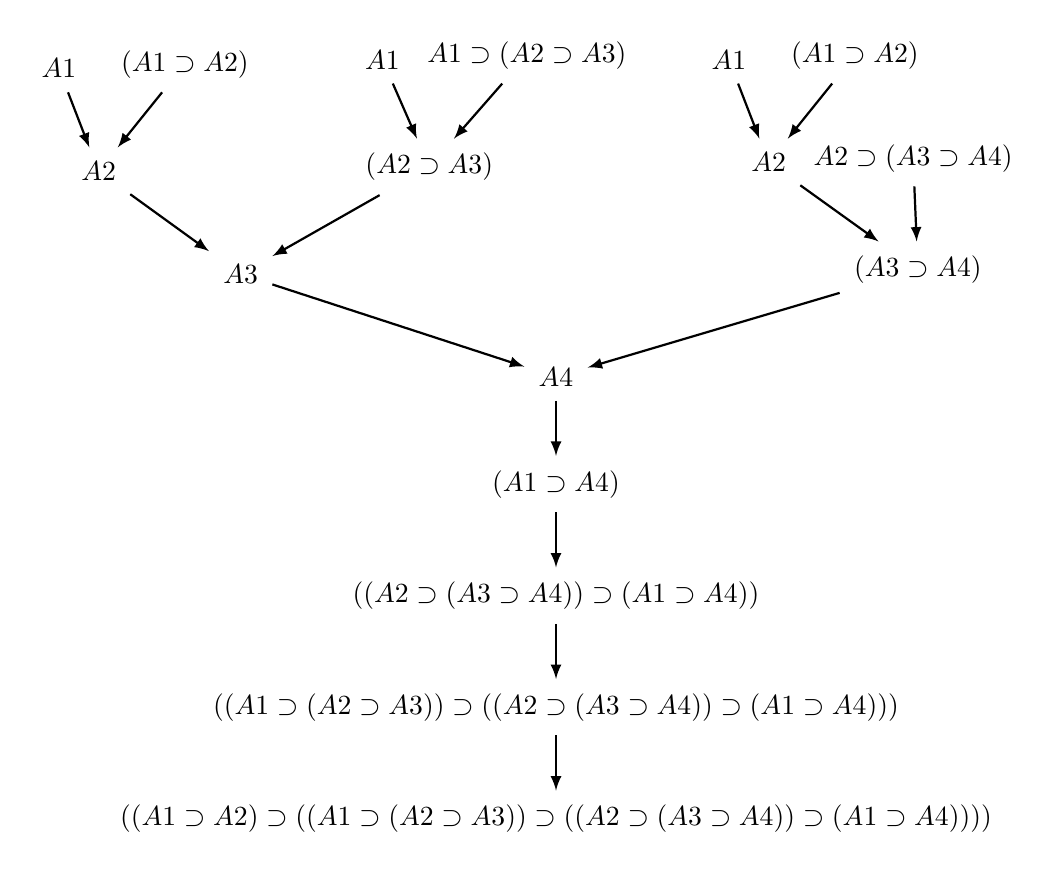
\begin{tikzpicture}[state/.style={rectangle, inner sep=5pt},  node distance=1cm]
            % \tikzstyle{every state}=[circle,thick,minimum size=5mm, text=black,minimum width=1cm]
            \node[state] (C1) {$((A1 \supset A2) \supset ((A1 \supset (A2 \supset A3)) \supset ((A2 \supset (A3 \supset A4)) \supset (A1 \supset A4))))$};
            \node[state] (C2) [above = 0.7cm of C1] {$((A1 \supset (A2 \supset A3)) \supset ((A2 \supset (A3 \supset A4)) \supset (A1 \supset A4)))$};
            \node[state] (C3) [above = 0.7cm of C2] {$((A2 \supset (A3 \supset A4)) \supset (A1 \supset A4))$};
            \node[state] (C4) [above = 0.7cm of C3] {$(A1 \supset A4)$};
            \node[state] (C5) [above = 0.7cm of C4] {$A4$};
            \node[state] (A3) [above left = 0.7cm and 3.2cm of C5] {$A3$};
            \node[state] (A3A4) [above right = 0.7cm and 3.2cm of C5] {$(A3 \supset A4)$};
            \node[state] (A2) [above left = 0.7cm and 1cm of A3] {$A2$};
            \node[state] (A2A3) [above right = 0.7cm and 1cm of A3] {$(A2 \supset A3)$};
            \node[state] (A1_1) [above left = 0.7cm and -0.3cm of A2] {$A1$};
            \node[state] (A1A2_1) [above right = 0.7cm and -0.3cm of A2] {$(A1 \supset A2)$};
            \node[state] (A1_2) [above left = 0.7cm and -0.8cm of A2A3] {$A1$};
            \node[state] (A1A2A3) [above right = 0.7cm and -1.2cm of A2A3] {$A1 \supset (A2 \supset A3)$};
            \node[state] (A2_2) [above left = 0.7cm and 0.5cm of A3A4] {$A2$};
            \node[state] (A2A3A4) [above right = 0.7cm and -2.5cm of A3A4] {$A2 \supset (A3 \supset A4)$};
            \node[state] (A1_3) [above left = 0.7cm and -0.3cm of A2_2] {$A1$};
            \node[state] (A1A2_2) [above right = 0.7cm and -0.3cm of A2_2] {$(A1 \supset A2)$};
            
            \path[-latex]  (C2) edge [thick, left] (C1);
            \path[-latex]  (C3) edge [thick, left] (C2);
            \path[-latex]  (C4) edge [thick, left] (C3);
            \path[-latex]  (C5) edge [thick, left] (C4);
            \path[-latex]  (A3) edge [thick, left] (C5);
            \path[-latex]  (A3A4) edge [thick, left] (C5);
            \path[-latex]  (A2) edge [thick, left] (A3);
            \path[-latex]  (A2A3) edge [thick, left] (A3);
            \path[-latex]  (A1_1) edge [thick, left] (A2);
            \path[-latex]  (A1A2_1) edge [thick, left] (A2);
            \path[-latex]  (A1_2) edge [thick, left] (A2A3);
            \path[-latex]  (A1A2A3) edge [thick, left] (A2A3);
            \path[-latex]  (A2_2) edge [thick, left] (A3A4);
            \path[-latex]  (A2A3A4) edge [thick, left] (A3A4);
            \path[-latex]  (A1_3) edge [thick, left] (A2_2);
            \path[-latex]  (A1A2_2) edge [thick, left] (A2_2);
            
            % \path[-latex]  (a1_2) edge [thick, left] node {0} (a2_2);
            % \path[-latex]  (a1a2_2) edge [thick, right] node {0} (a2_2);
            % \path[-latex]  (a2_2) edge [thick, left] node {0} (a3a4);
            % \path[-latex]  (a3a4) edge [thick, left, dotted] (sa3a4);
        \end{tikzpicture}
        \caption{EGDD da derivação de $Fib_4$}
        \label{fig:der_fib4}
    \end{center}
\end{figure}

Neste Capítulo utilizamos como métrica para o tamanho de uma prova o tamanho do grafo direcionado que o representa (\textit{quantidade de vértices} $+$ \textit{quantidade de arestas}).

O grafo que representa a prova de $Fib_4$ possui tamanho 40 (17 \textit{vértices} $+$ 16 \textit{arestas dedutivas} $+$ 7 \textit{arestas de descarte}), antes de iniciar a compressão, as arestas de descarte são substituídas pelas cadeias de bits de dependências associadas a cada aresta dedutiva, logo, o tamanho do grafo antes de inciar a compressão é 33.

% Na dedutiva, o t. A representação em DOT da prova possui xxx caracteres.aresta compressão da prova de $Fib_4$ são executados 4 colapsos de vértices. Considerando o nível da conclusão como o nível 1, até o nível 6 nenhum colapso é realizado; no nível 7, existem 2 vértices rotulados com 'A2' resultando em 1 colapso; no nível 8, existem 3 vértices rotulados com 'A2' resultando em 2 colapsos e existem 2 vértices rotulados com '$A1 \supset A2$' resultando em 1 colapso.

Considerando o nível da conclusão como o nível 1, o primeiro colapso é realizado no nível 7 entre os 2 vértices rotulados com a fórmula 'A2'.

\begin{center}
    \begin{tikzpicture}[state/.style={rectangle, inner sep=5pt},  node distance=1cm]
        % \tikzstyle{every state}=[circle,thick,minimum size=5mm, text=black,minimum width=1cm]
        \node[state] (a3) {$A3$};
        \node[circle,fill,inner sep=1.5pt] (sa3) [below = 1cm of a3] {};
        \node[state] (a2_1) [above = 1cm of a3] {$\boldsymbol{A2}$};
        \node[state] (a1_1) [above left = 1.25cm and 0cm of a2_1] {$A1$};
        \node[state] (a1a2_1) [above right = 1.25cm and 0cm of a2_1] {$A1 \mysupset A2$};
        
        \node[state] (a3a4) [right = 4cm of a3] {$A3 \supset A4$};
        \node[circle,fill,inner sep=1.5pt] (sa3a4) [below = 1cm of a3a4] {};
        \node[state] (a2_2) [above = 1cm of a3a4] {$\boldsymbol{A2}$};
        \node[state] (a1_2) [above left = 1.25cm and 0cm of a2_2] {$A1$};
        \node[state] (a1a2_2) [above right = 1.25cm and 0cm of a2_2] {$A1 \mysupset A2$};
        
        \path[-latex]  (a1_1) edge [thick, left] node {0} (a2_1);
        \path[-latex]  (a1a2_1) edge [thick, right] node {0} (a2_1);
        \path[-latex]  (a2_1) edge [thick, left] node {0} (a3);
        \path[-latex]  (a3) edge [thick, left, dotted] (sa3);
        
        \path[-latex]  (a1_2) edge [thick, left] node {0} (a2_2);
        \path[-latex]  (a1a2_2) edge [thick, right] node {0} (a2_2);
        \path[-latex]  (a2_2) edge [thick, left] node {0} (a3a4);
        \path[-latex]  (a3a4) edge [thick, left, dotted] (sa3a4);
    \end{tikzpicture}
\end{center}

\noindent Como ambos os vértices possuem 2 premissas e ainda não foram colapsados, são adicionadas 4 arestas de ancestralidade.

\begin{center}
    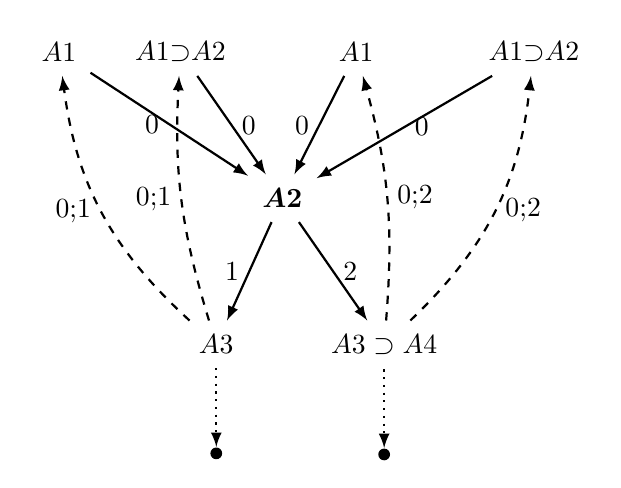
\begin{tikzpicture}[state/.style={rectangle, inner sep=5pt},  node distance=1cm]
        % \tikzstyle{every state}=[circle,thick,minimum size=5mm, text=black,minimum width=1cm]
        \node[state] (a2) {$\boldsymbol{A2}$};
        
        \node[state] (a3) [below left = 1.25cm and 0cm of a2] {$A3$};
        \node[state] (a3a4) [below right = 1.25cm and 0cm of a2] {$A3 \supset A4$};
        \node[circle,fill,inner sep=1.5pt] (sa3) [below = 1cm of a3] {};
        \node[circle,fill,inner sep=1.5pt] (sa3a4) [below = 1cm of a3a4] {};
        
        \node[state] (a1_1) [above left = 1.25cm and 2cm of a2] {$A1$};
        \node[state] (a1a2_1) [above left = 1.25cm and 0.1cm of a2] {$A1 \mysupset A2$};
        \node[state] (a1_2) [above right = 1.25cm and 0.1cm of a2] {$A1$};
        \node[state] (a1a2_2) [above right = 1.25cm and 2cm of a2] {$A1 \mysupset A2$};
        
        \path[-latex]  (a1_1) edge [thick, left] node {0} (a2);
        \path[-latex]  (a1a2_1) edge [thick, right] node {0} (a2);
        \path[-latex]  (a2) edge [thick, left] node {1} (a3);
        \path[-latex]  (a3) edge [thick, left, dotted] (sa3);
        
        \path[-latex]  (a1_2) edge [thick, left] node {0} (a2);
        \path[-latex]  (a1a2_2) edge [thick, right] node {0} (a2);
        \path[-latex]  (a2) edge [thick, right] node {2} (a3a4);
        \path[-latex]  (a3a4) edge [thick, left, dotted] (sa3a4);
        
        \path[-latex] (a3) edge [thick, left, dashed, bend left=20] node {0;1} (a1_1);
        \path[-latex] (a3) edge [thick, left, dashed, bend left=10] node {0;1} (a1a2_1);
        
        \path[-latex] (a3a4) edge [thick, right, dashed, bend right=10] node {0;2} (a1_2);
        \path[-latex] (a3a4) edge [thick, right, dashed, bend right=20] node {0;2} (a1a2_2);
    \end{tikzpicture}
\end{center}
 
No nível 8, o primeiro de dois colapsos dos vértices rotulados com 'A1' é realizado com os dois vértices que possuem uma aresta dedutiva apontando para o vértice rotulado com 'A2', colapsado no nível inferior. Ambos os vértices são premissas e cada um possui uma aresta de ancestralidade incidente.

\begin{center}
    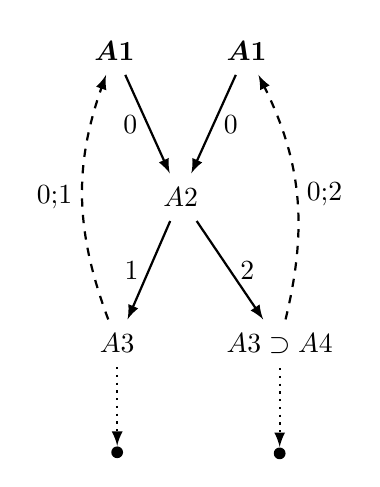
\begin{tikzpicture}[state/.style={rectangle, inner sep=5pt},  node distance=1cm]
        % \tikzstyle{every state}=[circle,thick,minimum size=5mm, text=black,minimum width=1cm]
        \node[state] (a2) {$A2$};
        \node[state] (a1_1) [above left =  1.25cm and 0cm of a2] {$\boldsymbol{A1}$};
        \node[state] (a1_2) [above right =  1.25cm and 0cm of a2] {$\boldsymbol{A1}$};
        \node[state] (a3) [below left =  1.25cm and 0cm of a2] {$A3$};
        \node[state] (a3a4) [below right =  1.25cm and 0cm of a2] {$A3 \supset A4$};
        
        \node[circle,fill,inner sep=1.5pt] (sa3) [below = 1cm of a3] {};
        \node[circle,fill,inner sep=1.5pt] (sa3a4) [below = 1cm of a3a4] {};
        
        \path[-latex]  (a1_1) edge [thick, left] node {0} (a2);
        \path[-latex]  (a1_2) edge [thick, right] node {0} (a2);
        \path[-latex]  (a3) edge [thick, left, dotted] (sa3);
        \path[-latex]  (a3a4) edge [thick, left, dotted] (sa3a4);
        \path[-latex]  (a2) edge [thick, left] node {1} (a3);
        \path[-latex]  (a2) edge [thick, right] node {2} (a3a4);
        \path[-latex]  (a3) edge [thick, left, dashed, bend left = 20] node {0;1} (a1_1);
        \path[-latex]  (a3a4) edge [thick, right, dashed, bend right = 20] node {0;2} (a1_2);
    \end{tikzpicture}
\end{center}

\noindent Além do colapso dos vértices, as arestas dedutivas que possuem o vértice 'V2' como destino também são colapsadas. A aresta colapsada é rotulada com a cor especial $\lambda$ e com as cores das arestas dedutivas colapsadas, que nesse caso é somente a cor 0. Como os vértices não possuem premissas, as arestas de ancestralidade incidentes são rebaixadas e seus respectivos rótulos são atualizados.

\begin{center}
    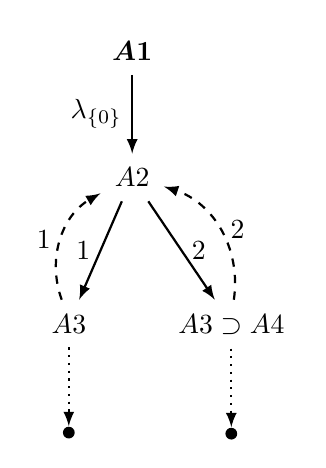
\begin{tikzpicture}[state/.style={rectangle, inner sep=5pt},  node distance=1cm]
        % \tikzstyle{every state}=[circle,thick,minimum size=5mm, text=black,minimum width=1cm]
        \node[state] (a2) {$A2$};
        \node[state] (a1_1) [above =  1cm of a2] {$\boldsymbol{A1}$};
        \node[state] (a3) [below left =  1.25cm and 0cm of a2] {$A3$};
        \node[state] (a3a4) [below right =  1.25cm and 0cm of a2] {$A3 \supset A4$};
        
        \node[circle,fill,inner sep=1.5pt] (sa3) [below = 1cm of a3] {};
        \node[circle,fill,inner sep=1.5pt] (sa3a4) [below = 1cm of a3a4] {};
        
        \path[-latex]  (a1_1) edge [thick, left] node {$\lambda_{\{0\}}$} (a2);
        \path[-latex]  (a3) edge [thick, left, dotted] (sa3);
        \path[-latex]  (a3a4) edge [thick, left, dotted] (sa3a4);
        \path[-latex]  (a2) edge [thick, left] node {1} (a3);
        \path[-latex]  (a2) edge [thick, right] node {2} (a3a4);
        \path[-latex]  (a3) edge [thick, left, dashed, bend left = 40] node {1} (a2);
        \path[-latex]  (a3a4) edge [thick, right, dashed, bend right = 40] node {2} (a2);
    \end{tikzpicture}
\end{center}

O vértice resultante do colapso anterior é colapsado com o outro vértice rotulado com 'A1' no nível 8 e que também não possui premissas. O vértice 'A2' possui 2 arestas de ancestralidade incidentes, mas elas não interferem no colapso. 

\begin{center}
    \begin{tikzpicture}[state/.style={rectangle, inner sep=5pt},  node distance=1cm]
        % \tikzstyle{every state}=[circle,thick,minimum size=5mm, text=black,minimum width=1cm]
        \node[state] (a1_1) {$\boldsymbol{A1}$};
        \node[state] (a2) [below =  1cm of a1_1] {$A2$};
        \node[circle,fill,inner sep=1.5pt] (sa2) [below = 1cm of a2] {};
        
        \node[state] (a1_2) [right =  4cm of a1_1] {$\boldsymbol{A1}$};
        \node[state] (a2a3) [below =  1cm of a1_2] {$A2 \supset A3$};
        \node[circle,fill,inner sep=1.5pt] (sa2a3) [below = 1cm of a2a3] {};
        
        \path[-latex]  (a1_1) edge [thick, left] node {$\lambda_{\{0\}}$} (a2);
        \path[-latex]  (a2) edge [thick, left, dotted] (sa2);
        
        \path[-latex]  (a1_2) edge [thick, left] node {0} (a2a3);
        \path[-latex]  (a2a3) edge [thick, left, dotted] (sa2a3);
    \end{tikzpicture}
\end{center}

\noindent Após o colapso, apenas um vértice é removido do grafo.

\begin{center}
    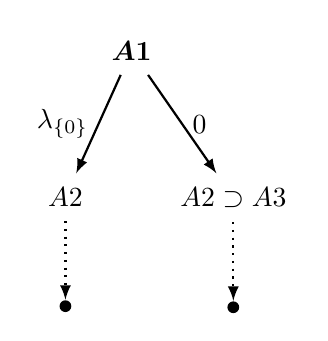
\begin{tikzpicture}[state/.style={rectangle, inner sep=5pt},  node distance=1cm]
        % \tikzstyle{every state}=[circle,thick,minimum size=5mm, text=black,minimum width=1cm]
        \node[state] (a1_1) {$\boldsymbol{A1}$};
        \node[state] (a2) [below left =  1.25cm and 0cm of a1_1] {$A2$};
        \node[circle,fill,inner sep=1.5pt] (sa2) [below = 1cm of a2] {};
        
        \node[state] (a2a3) [below right =  1.25cm and 0cm of a1_1] {$A2 \supset A3$};
        \node[circle,fill,inner sep=1.5pt] (sa2a3) [below = 1cm of a2a3] {};
        
        \path[-latex]  (a1_1) edge [thick, left] node {$\lambda_{\{0\}}$} (a2);
        \path[-latex]  (a2) edge [thick, left, dotted] (sa2);
        
        \path[-latex]  (a1_1) edge [thick, right] node {0} (a2a3);
        \path[-latex]  (a2a3) edge [thick, left, dotted] (sa2a3);
    \end{tikzpicture}
\end{center}

O último colapso, ainda no nível 8, envolve os dois vértices rotulados com $A1 \supset A2$. Ambos os vértices não possuem premissas e cada um possui uma aresta de ancestralidade incidente.

\begin{center}
    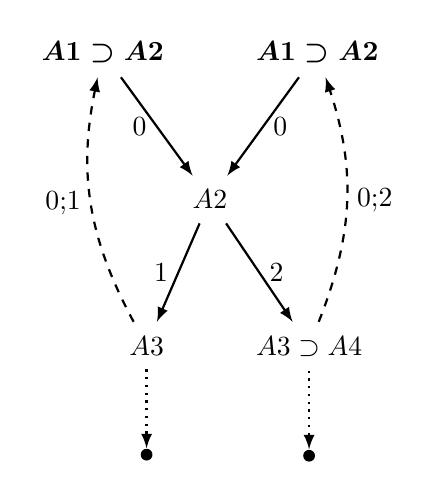
\begin{tikzpicture}[state/.style={rectangle, inner sep=5pt},  node distance=1cm]
        % \tikzstyle{every state}=[circle,thick,minimum size=5mm, text=black,minimum width=1cm]
        \node[state] (a2) {$A2$};
        \node[state] (a1_1) [above left =  1.25cm and 0cm of a2] {$\boldsymbol{A1 \supset A2}$};
        \node[state] (a1_2) [above right =  1.25cm and 0cm of a2] {$\boldsymbol{A1 \supset A2}$};
        \node[state] (a3) [below left =  1.25cm and 0cm of a2] {$A3$};
        \node[state] (a3a4) [below right =  1.25cm and 0cm of a2] {$A3 \supset A4$};
        
        \node[circle,fill,inner sep=1.5pt] (sa3) [below = 1cm of a3] {};
        \node[circle,fill,inner sep=1.5pt] (sa3a4) [below = 1cm of a3a4] {};
        
        \path[-latex]  (a1_1) edge [thick, left] node {0} (a2);
        \path[-latex]  (a1_2) edge [thick, right] node {0} (a2);
        \path[-latex]  (a3) edge [thick, left, dotted] (sa3);
        \path[-latex]  (a3a4) edge [thick, left, dotted] (sa3a4);
        \path[-latex]  (a2) edge [thick, left] node {1} (a3);
        \path[-latex]  (a2) edge [thick, right] node {2} (a3a4);
        \path[-latex]  (a3) edge [thick, left, dashed, bend left = 20] node {0;1} (a1_1);
        \path[-latex]  (a3a4) edge [thick, right, dashed, bend right = 20] node {0;2} (a1_2);
    \end{tikzpicture}
\end{center}

\noindent Esse colapso é semelhante ao primeiro colapso dos vértices $A1$, no entanto, as arestas de ancestralidade são removidas em vez de serem rebaixadas, pois, já existem arestas de ancestralidade de A3 para A2, e de $A3 \supset A4$ para A2 com os mesmos rótulos. Esse colapso remove 3 arestas, sendo 1 dedutiva e 2 de ancestralidade.

\begin{center}
     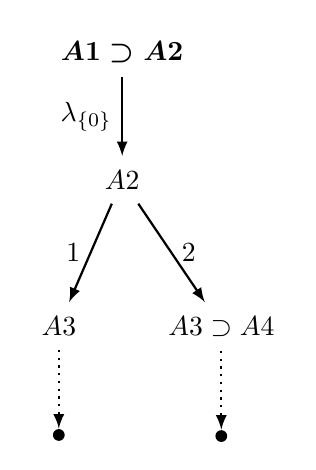
\begin{tikzpicture}[state/.style={rectangle, inner sep=5pt},  node distance=1cm]
        % \tikzstyle{every state}=[circle,thick,minimum size=5mm, text=black,minimum width=1cm]
        \node[state] (a2) {$A2$};
        \node[state] (a1_1) [above =  1cm of a2] {$\boldsymbol{A1 \supset A2}$};
        \node[state] (a3) [below left =  1.25cm and 0cm of a2] {$A3$};
        \node[state] (a3a4) [below right =  1.25cm and 0cm of a2] {$A3 \supset A4$};
        
        \node[circle,fill,inner sep=1.5pt] (sa3) [below = 1cm of a3] {};
        \node[circle,fill,inner sep=1.5pt] (sa3a4) [below = 1cm of a3a4] {};
        
        \path[-latex]  (a1_1) edge [thick, left] node {$\lambda_{\{0\}}$} (a2);
        \path[-latex]  (a3) edge [thick, left, dotted] (sa3);
        \path[-latex]  (a3a4) edge [thick, left, dotted] (sa3a4);
        \path[-latex]  (a2) edge [thick, left] node {1} (a3);
        \path[-latex]  (a2) edge [thick, right] node {2} (a3a4);
    \end{tikzpicture}
\end{center}

A Tabela \ref{tab:col_tam} mostra o tamanho do grafo em cada colapso. Apesar de não ser a métrica que descreve o real de tamanho da prova, pois são adicionadas informações às arestas durante a compressão, o tamanho do grafo evidencia o comportamento da Compressão Horizontal durante a compressão de uma prova. Nos primeiros colapsos o tamanho do grafo de prova é superior ao tamanho do grafo antes da compressão, mas a medida que colapsos vão sendo executados e vértices e arestas são retirados, o tamanho do grafo tende a diminuir. 

\begin{table} [!ht]
    \caption{Tamanho do grafo direcionado em cada colapso}\label{tab:col_tam}
    ~\\[-2mm]
    \begin{tabularx}{\textwidth}{@{\extracolsep{0pt}}C @{\extracolsep{0pt}}C C}

        \textbf{Passo}
        & \textbf{Tamanho (vértices + arestas)}
        \\\toprule

        ~ \\[-6mm]
        grafo inicial
        & 33 (17 + 16)
        \\\midrule
    
        ~ \\[-6mm]
        colapso 1
        & 36 (16 + 20)
        \\\midrule
    
        ~ \\[-6mm]
        colapso 2
        & 34 (15 + 19)
        \\\midrule
    
        ~ \\[-6mm]
        colapso 3
        & 33 (14 + 19)
        \\\midrule
        
        ~ \\[-6mm]
        colapso 4
        & 29 (13 + 16)
        \\\midrule
    \end{tabularx}
\end{table}

O Capítulo \ref{cap:impl_exp} apresenta como os grafos de prova (EGDD) da Compressão Horizontal são representados em arquivos e o Capítulo \ref{cap:experimentos} apresenta os resultados de compressão utilizando a representação em arquivos de texto.
  % -*- coding: utf-8; -*-

\chapter{Estruturas para Provas em M$\supset$}
  % -*- coding: utf-8; -*-

\chapter{Resultados}
  % -*- coding: utf-8; -*-

\chapter{Conclusão e Trabalhos Futuros}
\label{cap:conc_trab}

Com o objetivo inicial de implementar a Compressão Horizontal e comparar seu desempenho na compressão de provas em dedução natural da M$\supset$ com outras técnicas de compressão relatadas na literatura, concluímos esta dissertação com o objetivo parcialmente atingido. Identificamos na literatura apenas a Dedução Natural Contextual \cite{NDcPaleo} como técnica de compressão de provas em dedução natural da $M\supset$, no entanto, seu provador \cite{paleo2015implementation} não foi capaz de gerar nenhuma prova das fórmulas selecionadas para o experimento.

Implementamos o \textit{compressing}, compressor de provas em Dedução Natural da M$\supset$ que utiliza o algoritmo da Compressão Horizontal, e propomos formatos e convenções para os arquivos que contêm as provas submetidas à compressão e para os arquivos que contêm as provas comprimidas. Projetamos o compressor como o padrão de projetos \textit{adapter} para que possíveis alterações de componentes externos (manipulação e visualização de grafos) sejam facilitadas.

Na preparação dos experimentos, selecionamos famílias de fórmulas na literatura com as características adequadas para mostrar a capacidade de compressão da Compressão Horizontal, ou seja, fórmulas que possuem provas grandes, preferencialmente, com tamanho exponencial em ralação ao tamanho da conclusão. Entre as famílias de fórmulas selecionadas, o provador utilizado, o NatDProver, gerou provas apenas para a $Fib_n$.

Nos resultados dos experimentos, reportamos as informações das execuções da Compressão Horizontal e da codificação de Huffman para as fórmulas de $Fib_n$. A Compressão obteve taxas de compressão de até 95\%, enquanto que a codificação de Huffman obteve aproximadamente 40\% de taxa de compressão para todas as provas.

Nossa principal contribuição é a implementação do \textit{compressing}, que implementa o algoritmo da Compressão Horizontal, capaz de comprimir qualquer prova da M$\supset$ para um tamanho polinomialmente limitado em relação ao tamanho da conclusão. Se qualquer tautologia da M$\supset$ possui provas com tamanho polinomialmente limitado, então $NP = PSPACE$. No entanto, a base de provas utilizadas para a obtenção dos resultados das taxa  de compressão é limitada, sendo composta apenas por fórmulas que compartilham a mesma estrutura. 

Listamos a seguir os possíveis trabalhos futuros:
\begin{itemize}
    \item Diversificar a base de provas para os experimentos do \textit{compressing}, adaptando um outro provador já existente ou corrigindo as falhas do NatDProver.
    \item Adicionar o algoritmo de verificação da Compressão Horizontal, que verifica se a derivação comprimida é válida, ao \textit{compressing}.
    \item Melhorar a interação do usuário com o \textit{compressing}, implementando uma interface por linha de comando.
    \item Otimizar os algoritmos internos do \textit{compressing} para melhorar os resultados de tempos de execução.
\end{itemize}

  \arial
  \bibliography{flavio}
\end{document}
